\documentclass[format=acmsmall, review]{acmart}
\settopmatter{printfolios=true,printccs=false,printacmref=false}

\usepackage{booktabs} % For formal tables
%% \usepackage{alltt}
\usepackage{longtable}
\usepackage{tabu}
\usepackage{alltt}
\usepackage[utf8]{inputenc}

%% Metadata Information
\copyrightyear{2018}
%%\acmArticleSeq{9}
\acmNumber{HOPL} % CONF = POPL or ICFP or OOPSLA

%% Copyright
%%\setcopyright{acmcopyright}
%% \setcopyright{acmlicensed}
\setcopyright{rightsretained}
%%\setcopyright{usgov}
%%\setcopyright{usgovmixed}
%%\setcopyright{cagov}
%%\setcopyright{cagovmixed}
\usepackage{natbib}
\citestyle{acmauthoryear}

%% Paper history
\received{August 2018}

%% While Richard prefers "Emacs Lisp" I find it unnecessarily verbose
%% and much prefer "Elisp" which is also very widely used.
\newcommand \Elisp {Emacs Lisp}
\newcommand \MAlign [1] {\begin{array}{@{}l@{}}#1\end{array}}
\newcommand \id[1] {\textrm{\textsl{#1}}}

%% Document starts
\begin{document}
%% Title portion. Note the short title for running heads
\title{Evolution of Emacs Lisp}

\author{Stefan Monnier}
\affiliation{%
  \institution{Université de Montréal}
  \streetaddress{C.P.\ 6128, succ.\ centre-ville}
  \city{Montréal}
  \state{QC}
  \postcode{H3C 3J7}
  \country{Canada}}
\email{monnier@iro.umontreal.ca}
\author{Michael Sperber}
\affiliation{%
  \institution{Active Group GmbH}
  \streetaddress{Hechinger Str.\ 12/1}
  \city{Tübingen}
  \country{Germany}
}
\email{sperber@deinprogramm.de}


\input abstract

\ccsdesc{Social and professional topics}
\ccsdesc{Professional topics}
\ccsdesc{History of computing}
\ccsdesc{History of programming languages}

%%
%% End generated code
%%


\keywords{history of programming languages, Lisp, Emacs Lisp}


\maketitle

\tableofcontents

\section{Introduction}

Emacs is a text editor originally developed by Richard Stallman, who is also
the founder of the Free Software Foundation (FSF) and who launched the GNU
Project.

\Elisp{} is the extension language of the Emacs text editor.
In this sense, it is just a side-project of Emacs and might be overlooked as
a programming language.  But Emacs itself comes with more than a million
lines of \Elisp{} code, and yet more \Elisp{} is distributed separately from
Emacs in various Emacs Lisp Package Archives (ELPA).  If you additionally
consider that the majority of Emacs users have likely written a few lines of
\Elisp{} in their configuration file, it is arguably one of the most widely
used dialects of Lisp.

%% FIXME: I feel like we should add something here, but not sure what.

\subsection{The authors}

Neither of us was around when Emacs and \Elisp{} were designed, but we are
two researchers in programming languages with a keen interest and many
years of
experience in (X)Emacs and \Elisp{}, which made us well positioned to write
this article.

\smallskip

\noindent{Stefan Monnier} has been (and is still) a core contributor to
Emacs since 1999, was head maintainer from 2008 to 2015, and he supervised
student projects on the \Elisp{} implementation in Emacs.

\smallskip

\noindent{Michael Sperber} has been a core contributor to XEmacs since 1994.
Most of his work was done from 1995 to 2003, when he was a research
assistant at the University of Tübingen.  Apart from his own work on
the XEmacs codebase, he supervised several student projects on the
\Elisp{} implementation in XEmacs, including a co-authored paper on the
analysis of dynamic scope~\cite{Neubauer01}.

\subsection{Paper organization}

\Elisp{} has evolved in several strands and implementations over the
years, and thus its evolution did not happen along a single timeline.
Moreover, some aspects evolved over long periods of time.  To avoid
excessive interleaving of those aspects, we have organized the
top-level structure of the paper into chronological eras.  Within an
era, as a new topic is introduced, we usually follow that topic
chronologically to its conclusion, even if that means going beyond the
era where it started.

Emacs as we know it today itself started in 1984.
Section~\ref{sec:early-history} describes the driving motivation for
the early design and implementation of \Elisp.  The following Section
\ref{sec:base-language-design} traces the evolution of the base
language design, and Section \ref{sec:base-language-implementation}
its implementation.
Development continued at a high pace until about 1991.
Around that time, its development slowed down and
was overtaken by Lucid Emacs, later renamed XEmacs, whose impact on
\Elisp{} we describe in Section~\ref{sec:xemacs}.  Eventually,
development of Emacs picked up again, and both co-evolved until about
2007.  We describe the relevant aspects of that evolution in
Section~\ref{sec:coevolution}.  After 2007, XEmacs development slowed
down, and we describe this post-XEmacs period in
Section~\ref{sec:post-xemacs}, to finally conclude in
Section~\ref{sec:conclusion}.

\Elisp{} was re-implemented in several other projects outside this
succession.  We briefly touch upon those projects in
Appendix~\ref{sec:alternative-implementations}.  

\section{Emacs history}
\label{sec:emacs-history}

While in theory \Elisp{} exists independently from Emacs, its design,
implementation, and history are inextricably linked to that of Emacs, so we
present here a short overview of the important events in Emacs's life.

\subsection{Emacs's early history}
\label{sec:emacs-early-history}

Emacs's original inception was as a set of macros and keybindings for the
TECO text editor.  TECO was written by Dan Murphy starting in
1962~\cite{Murphy09}, then at the MIT AI lab, and featured a primitive
programming language~\cite{Stallman2018-personal}.  In the mid-1970s Richard
Stallman, then also at MIT, added to TECO a ``real-time edit mode'' (then
a novelty), which updated the display of the text being edited as typing
happened~\cite{MulticsEmacs1996}.  This mode allowed mapping characters to little TECO programs, and
users would typically configure TECO to bind printing characters to
self-insert, and control characters to perform other tasks such as
navigation to other parts of the text via so-called \textit{macros}.  Guy Steele
coordinated among the users, creating a common set of keybindings and macros, which
Richard Stallman evolved into the first version of
Emacs~\cite{EmacsLore,Seibel2009}.  (``Emacs'' stands for ``editor macros.'')
Note that TECO and Emacs were not completely separate entities in the sense
that TECO's extension language was also Emacs's extension language and that
they evolved together, where TECO's extension language was regularly
extended to provide facilities then used by Emacs~\cite{Stallman2002}.

This original Emacs grew popular in the lab and soon started to be
reimplemented in various other systems.  Several of those incarnations of
Emacs were written in Lisp, notably \emph{EINE} (recursive acronym for
``EINE Is Not Emacs'') on the Lisp Machine by Dan Weinreb, followed by
\emph{ZWEI} (for ``ZWEI was EINE Initially'') by Dan Weinreb and Mike
McMahon~\cite{Weinreb1979}), and \emph{Multics Emacs} by Bernie Greenberg in
1978~\cite{MulticsEmacs1996,Stallman2002} written in MacLisp~\cite{Moon1974,Pitman1983}.
Given Lisp's dynamic nature, it was only natural that those systems used
Lisp as their extension language.

\emph{Unix Emacs}, written by James Gosling in 1980/1981~\cite{Gosling1981}
and preserved in the history books as \emph{Gosling Emacs},
was implemented in C and it featured an extension
language called \emph{MLisp} or \emph{Mock Lisp}, which bears visual
resemblance to Lisp, but was a lesser member of the Lisp family in the
sense that it lacked data structures like \emph{cons} cells and was
generally too limited to be usable as an implementation language.

Richard Stallman, who had worked on
ZWEI~\cite{Stallman2018-personal}, liked the possibilities offered for
extending the editor by having Lisp be both the extension language and the
implementation language.  But high-performance Lisp compilers were not
widely available, so he decided to write a (for him) second version of Emacs
which would use Lisp as its extension language, like Greenberg's Multics
Emacs, but where the implementation would be partly written in Lisp and
partly in C (including buffer manipulation primitives, the redisplay code,
and a Lisp interpreter) so as to be more widely available.

In 1984, Richard Stallman took Gosling Emacs as a starting point for this
endeavor, and began replacing
the \emph{Mock Lisp} interpreter and data structures of Gosling Emacs
with a new interpreter for the language that is now \Elisp{}, adapting
internal data structures to those of
this \Elisp{} interpreter.  At that time, Gosling Emacs was distributed
commercially by Unipress under the name \emph{Unipress Emacs}, and Unipress
ordered Richard Stallman to stop distributing his version of Emacs, which
forced him to replace or rewrite the rest of Emacs's code as well, such as
the code responsible for the redisplay.  It also motivated him to invent the
GNU General Public License \cite{GPLHistory}, to try and ensure that users
of his code would never have to go through such an experience.

\subsection{Design goals}

The initial design of \Elisp{} was motivated by the pervasive requirement of
\emph{extensibility}: users ``must be able to redefine each
character''~\cite{Stallman1981}.  TECO and Gosling Emacs featured small
languages that were either too obscure or too weak to support this vision.
Consequently, Richard Stallman took inspiration from MacLisp, and \Elisp{}
started right from the beginning as a full-featured programming language with
powerful abstraction facilities, thus foregoing Greenspun's tenth
rule, a popular epigram on programming that came up in  1993: ``Any
sufficiently complicated C or Fortran program contains an
ad-hoc, informally-specified, bug-ridden, slow implementation of half of
Common Lisp.''~\cite{GreenspunsRule}

Moreover, Richard Stallman made the design of Emacs embody and showcase
the ideals of Free Software.  For example, not only is it permitted to get
and modify the source code, but every effort is made to encourage the
end-user to do so.  The resulting requirements had a profound influence on
the \Elisp{} language.  Retrospectively, those
can be summarized as:
\begin{itemize}
\item The language should be accessible to a wide audience, so that as many
  people as possible can adapt Emacs to their own needs, without being
  dependent on the availability of someone with technical expertise.
  For example, the
  \emph{Introduction to Programming in Emacs Lisp}
  tutorial~\citep{ElispIntro} targets users with no programming
  experience.  This has been a strong motivation to keep \Elisp{} on the
  minimalist side and to resist incorporation of many Common Lisp features.
\item It should be easy for the end-user to find the relevant code in order
  to modify Emacs's behavior.  This has driven the development of elements
  such as the \emph{docstrings} (Section~\ref{sec:docstrings}) and more generally the self-documenting
  aspect of the language.  It also imposes constraints on the evolution of
  the language: the use of some facilities, such as \emph{advice}
  (Section~\ref{sec:advice}), is
  discouraged because it makes the code more opaque.
\item Emacs should be easily portable to as many platforms as possible.
  This largely explains why \Elisp{} still runs in a simple byte-code interpreter.
\end{itemize}

\subsection{The great schism}
\label{sec:schism}
%% Note: I put "1988" here based on Richard Gabriel's email (quoted in
%% https://www.jwz.org/doc/lemacs.html) from 22 Jun 1992 where he says "4
%% years ago".
In 1988, Lucid Inc., a software development company founded by Richard
Gabriel and based in Menlo
Park, California, started a project called \emph{Energize}~\cite{GabrielEtAl1990,Gabriel-personal}.
Energize was to be a C/C++ integrated development environment based on
Emacs~\cite{GabrielLetter}.  Lucid decided to use Emacs as the central
component of Energize.  At the time, the current version of Emacs was
18, which was still essentially a textual application.
For Energize, Lucid needed a graphical user
interface and the ability to add a large number of annotations to
program source code.

Lucid hired Joseph Arcenaux,
the principal Emacs developer at that time, to add these features
for Lucid while continuing to work on the upcoming release of Emacs
19.  It soon became clear that the respective goals Lucid and the Free
Software Foundation had for Emacs 19 were incompatible,
and the required cooperation between Lucid and
the Free Software Foundation broke down~\cite{Arcenaux-interview}.

As a result, Lucid forked Emacs development, creating its own Emacs
variant \emph{Lucid Emacs}, whose primary developer and maintainer was
Jamie Zawinski.

In 1994, Lucid went bankrupt.  Sun subsequently wanted to ship
Lucid Emacs with their operating system, and ended up financing some
of the continued development of Lucid Emacs, and effected a name
change to the current \emph{XEmacs}.
Sun eventually lost interest in XEmacs, which continued as an
open-source community effort.

\subsection{Timeline}

\newcommand \EDate [2] {#1}     %Ignore second argument (day) to save space.

\begin{table}
  \caption{Emacs development timeline}
  \label{tab:timeline}
\begin{center}
  \begin{tabular}{@{}l|l|l|l}
    Date & Version & Maintainer & Notes \\ \hline
    \EDate{1985-03}{-20}
    & Emacs 13 & Richard Stallman & Earliest recorded release \\
    \EDate{1985-07}{-15}
    & Emacs 16.56 & Richard Stallman
    & Oldest version still available \\
    &&& Gosling Emacs code expunged\\
    \EDate{1987-09}{-18} & Emacs 18.49 & Richard Stallman \\
    1987 & Epoch & Alan M.\ Carroll & Forks from Emacs 18.49\\
    \EDate{1988-12}{-14} & Epoch 1.0 & Alan M.\ Caroll, Simon Kaplan\\
    \EDate{1989-08}{-23} & Emacs 18.55 & Richard Stallman \\
    1990 & Emacs 19 & Joe Arcenaux & Forks from Emacs 18.55 \\
    &&& Text properties, Sec.~\ref{sec:strings};\\
    &&& \texttt{advice.el}, Sec.~\ref{sec:hooks} \\
    1990-04 & Lucid Emacs 19.0 & Jamie Zawinski & Extents, Sec.~\ref{sec:strings} \\
    \EDate{1990-08}{-27} & Epoch 4.0 & Marc Andreesen \\
    \EDate{1992-10}{-31} & Emacs 18.59 & Richard Stallman
    & Last release of Emacs 18\\
    \EDate{1993-05}{-22} & Emacs 19.7 beta & Jim Blandy & First public beta of Emacs 19 \\
    &&& \texttt{lambda} macro, Sec.~\ref{sec:lambda}\\
    \EDate{1993-05}{-27} & Emacs 19.8 beta & Jim Blandy \\
    \EDate{1993-09}{-06} & Lucid Emacs 19.8 & Jamie Zawinski
    & 4-bit tags, Sec~\ref{sec:data-representation} \\
    &&& Merged Epoch and Emacs 19.8 \\
    \EDate{1994-05}{-17} & Emacs 19.23 beta & Richard Stallman \\
    \EDate{1994-05}{-27} & Lucid Emacs 19.10 & Jamie Zawinski \\
    \EDate{1994-09}{-13} & XEmacs 19.11 & Chuck Thompson, Ben Wing \\
    \EDate{1994-11}{-01} & Emacs 19.28 & Richard Stallman
    & Proper backquote, Sec.~\ref{sec:backquote} \\
    &&& First real release of Emacs 19\\
    \EDate{1995-06}{-19} & Emacs 19.29 & Richard Stallman
    & 3-bit tags, Sec.~\ref{sec:data-representation} \\
    1995 & XEmacs 20 && Work on MULE support begins\\
    \EDate{1995-09}{-01} & XEmacs 19.13 & Chuck Thompson, Ben Wing
    & Merged Emacs 19.30\\
    %% \EDate{1995-11}{-24} & Emacs 19.30 & Richard Stallman \\
    %% \EDate{1996-05}{-25} & Emacs 19.31 & Richard Stallman \\
    \EDate{1996-08}{-21} & Emacs 19.34 & Richard Stallman
    & Last release of Emacs-19 \\
    \EDate{1997-02}{-09} & XEmacs 20.0 & Steve Baur & Custom library,
    Sec.~\ref{sec:custom} \\
    \EDate{1997-03}{-26} & XEmacs 19.15 & Steve Baur \\
    \EDate{1997-09}{-17} & Emacs 20.1 & Richard Stallman
    & First release with MULE \\
    \EDate{1997-10}{-31} & XEmacs 19.16 & Steve Baur \\
    \EDate{1998-02}{-28} & XEmacs 20.4 & Steve Baur
    & First stable release with MULE\\ % support
    &&& Packages shipped separately\\
    \EDate{1998-07}{-12} & XEmacs 21.0 & Steve Baur & 1-bit tags \\
    \EDate{2001-04}{-16} & XEmacs 21.4 & Stephen Turnbull \\
    \EDate{2001-10}{-20} & Emacs 21.1 & Gerd Möllmann
    & New redisplay engine \\
    %% \EDate{2002-03}{-18} & Emacs 21.2 & Gerd Möllmann
    %% & Last version with MLisp support, Sec.~\ref{sec:mock-lisp}\\
    \EDate{2007-06}{-01} & Emacs 22.1 & Richard Stallman
    & Last bits of Mock Lisp removed \\
    %% Chong and I started as maintainers in February 2008.
    \EDate{2009-07}{-28} & Emacs 23.1 & Chong Yidong, Stefan Monnier
    & Unicode internally, Sec.~\ref{sec:unicode}  \\
    \EDate{2012-06}{-10} & Emacs 24.1 & Chong Yidong, Stefan Monnier
    & Lexical scoping, Sec.~\ref{sec:lexical-scoping}
      %% FIXME: No room on the same line, not sure it's worth using an
      %% extra line for it:
      %% ; Pcase, Sec.~\ref{sec:pcase}
      \\
    \EDate{2013-03}{-10} & Emacs 24.3 & Chong Yidong, Stefan Monnier
    & CL-Lib, Sec.~\ref{sec:cl-lib} \\
    \EDate{2014-10}{-20} & Emacs 24.4 & Chong Yidong, Stefan Monnier
    & \texttt{nadvice.el}, Sec.~\ref{sec:hooks}\\
    \EDate{2016-09}{-17} & Emacs 25.1 & John Wiegley, Eli Zaretskii \\
    \EDate{2018-05}{-28} & Emacs 26.1 & John Wiegley, Eli Zaretskii
    & Records, Sec.~\ref{sec:structures}; Threads, Sec~\ref{sec:concurrency} \\
    %% \EDate{20??-??}{-??} & Emacs 27 &
    %%     & Old-style backquotes removed, Sec.~\ref{sec:backquote} \\
  \end{tabular}
\end{center}
\end{table}

Table~\ref{tab:timeline} contains a timeline of significant milestones in
the development of Emacs and Lucid Emacs/XEmacs.  It also includes a few
milestones from \textit{Epoch}, a predecessor to Lucid Emacs that had
support for multiple windows.

For the time until 2007, the timeline in this table borrows much
from Jamie Zawinski's timeline~\cite{JWZTimeline}.
According to the \texttt{etc/NEWS.1-17} file, Emacs versions counted from
1.1 to 1.12 and then switched to 13 which was the first version announced
publicly on usenet.

\subsection{Development model}

This section describes the development organization of Emacs and Lucid
Emacs/XEmacs, respectively.

\paragraph{Emacs}
Emacs is a Free Software project, developed by a loosely connected
set of volunteers doing it mostly in their spare time, and several of them
do not consider themselves computer professionals.  Development is not
really organized, in the sense that volunteers work on what they find
appealing rather than follow some agreed upon plan, and the overall
direction of evolution is in effect controlled by the \emph{head
maintainer(s)} by accepting or rejecting contributions, and via discussions in
mailing-lists.  At times, the Free Software Foundation paid the
maintainer a salary, but this is not currently the case.

Richard Stallman was the original maintainer and still participates: even
though several other people have been official maintainers at various points
in time, he always acted as a ``default maintainer'' when no one wanted to
step up and he has followed Emacs's development very closely even when he
was not officially the maintainer.  Also, Richard Stallman being
the founder of the Free Software Foundation, Emacs is part of the FSF's GNU
project and is hence linked to the FSF by its use of FSF's resources to host
the code and own the copyright.  The link with the FSF is of course
particularly strong because of Stallman's role in Emacs.

The organization of Emacs's development is not really codified, but in
practice the role of the maintainer is a balancing act between the desire to
maintain a sane code base, to promote Free Software, to be attractive to its
users, and to encourage contributions.  There is also more structure to the
organization: maintenance is really shared among a handful of people who
earned each other's respect by the weight of their past contributions and
who can then make more or less any change they like to the code, and accept
or reject external contributions, as long as nobody complains.  In case of
disagreement between those core contributors the maintainer has the final
say.  This structure probably appeared around 1991 and until 2000 was
embodied in the fact that the core contributors were members of a private
\emph{emacs-core} mailing-list and were the only ones with direct access to
the code.  Since late 2000, when the CVS server became public and the
\emph{emacs-core} private mailing-list was replaced by the public
\emph{emacs-devel} mailing-list, this has become much more blurry:
technically, more than a hundred contributors have direct write access to
the code now and nowhere is it ever written or said which of those is or
isn't considered a core contributor at any given point it time.  Instead the
system functions by self-regulation: every time someone installs a change
without prior permission, someone else may or may not complain about the
change's quality, which can lead to requiring further changes or even
a complete revert, so over time contributors learn to judge on their own
what makes a change acceptable.

\paragraph{Lucid Emacs/XEmacs}
Lucid Emacs was initially managed by the respective maintainers, who
integrated patches sent by contributors, and published tarballs for
releases on ftp sites.

This changed when Steve Baur took over as maintainer in 1996: He
imported the source code into a publically accessible CVS repository on
the SourceForge platform for open-source software.  Steve Baur then
established a \textit{review board} whose members received commit
access to the repository, and whose job was to review and apply
patches via a special mailing list, \texttt{xemacs-patches}, which
exists to this day.

For XEmacs 19.15, Steve Baur also split off many \Elisp{} packages
into a separate repository, with the ability to manage and update the
packages independently from the core releases, and installed
individual maintainers for many of these packages.

In 2007, Michael Sperber migrated the source code from CVS to
Mercurial, hosted on the Bitbucket platform.

\section{Early language design}         % -1992?
\label{sec:early-history}

The design of \Elisp{} was based on the past experiences with the extension
languages of TECO, ZWEI, Gosling Emacs, and Multics Emacs.
Arguably, the strongest influence for the language itself was MacLisp while
the design of the editing primitives was influenced by Gosling Emacs's
Mock Lisp.

\subsection{Mock Lisp}
\label{sec:mock-lisp}

Gosling Emacs, arguably the immediate predecessor of today's Emacs,
featured an extension language called \emph{MLisp} or \emph{Mock Lisp},
which bears visual resemblance to \Elisp{}.  MLisp featured function
definitions via \texttt{defun}, as well as many built-in functions (such as
\texttt{eolp}, \texttt{forward-character}, \texttt{save-excursion}) whose
names survive in \Elisp{}.  Emacs even contained some limited
back\-ward-compatibility support for MLisp until Emacs 22 in 2007.

MLisp was a quite limited language: It lacked cons cells and lists.
MLisp did have dynamic scoping and local variables, but a peculiar
mechanism for passing arguments:  There were no named
parameters.  Instead, a program would invoke the \texttt{arg}
function: For example, \texttt{(arg 1)} would access the first
argument.  Moreover, argument expressions were essentially evaluated
in a call-by-name fashion by \texttt{arg}, and evaluation happened in
the dynamic environment of the callee.

With the design of the primitives, Richard Stallman adopted MLisp's
basic approach~\cite{Stallman2018-personal}, diverging from ZWEI.
ZWEI primitives would always take explicit arguments to specify what
text to operate on.  Here is what a ZWEI function might have looked
like that inserted a string surrounded by parentheses:
%
\begin{verbatim}
    (DEFUN INSERT-PARENS (BP STRING)
      (LET* ((BP1 (INSERT BP "("))
             (BP2 (INSERT BP1 STRING))
             (BP3 (INSERT BP2 ")")))
        BP3))
\end{verbatim}
%
The \texttt{BP} parameter is for the location at which the insertion
is to take place.  \texttt{INSERT-PARENS} calls the primitive
\texttt{INSERT} function three times; \texttt{INSERT} returns a new
location, after the insertion, which gets threaded through the
subsequent \texttt{INSERT} calls and finally returned.

The Mock Lisp primitives differed from those of ZWEI in that they operated
at the current \emph{point} (the current ``cursor position''), as was the
case in TECO.  Here is the \texttt{in-parens} function from the Gosling
Emacs manual~\cite{Gosling1981}:
%
\begin{verbatim}
    (defun
          (in-parens ; The name of the function.
            (insert-string "(")
            (insert-string (arg 1 "String to insert? "))
            (insert-string ")")
          )
          )
\end{verbatim}
%
Stallman, who had worked on ZWEI, found ZWEI's approach clumsy, and
used MLisp's approach for Emacs.

\subsection{Maclisp}

MacLisp was a Lisp dialect developed at MIT's Project MAC in the early
1970s, which was named for its conceptual relationship with ``Multiple
Access Computers'' and ``Machine-Aided Cognition''~\cite{Pitman1983}.
It was developed for use in artificial intelligence research and
related fields.  It descended from Lisp 1.5, albeit with many changes~\cite{Moon1974}.
MacLisp ran on the DEC PDP-10 series machines under various operating
systems, and on the Honeywell 6180/6880 under Multics.

Maclisp had all basic properties associated with Lisp today~\cite{Moon1974}:
%
\begin{itemize}
\item Structure is defined through parentheses and prefix notation.
\item Code forms have an internal representation as
  \textit{S-expressions}, which print the same as the code, a property called
  homoiconicity.
\item There is an \texttt{eval} function that evaluates an expression
  represented as an S-expression.
\item The basic data structure is \textit{cons}, which pairs two
  objects, with the first component named \textit{car}, the second
  \textit{cdr}.  Conses are used to implement singly-linked
  \textit{lists}, where a special \textit{nil} value indicates the end
  of the list.  Conses are mutable.
\item A special \textit{symbol} data type represents identifiers in
  S-expressions, but is also often used to represent enumeration,
  status values etc.
\item It is possible to define new compound data types via the
  \texttt{defstruct} form.
\item The language has first-class functions via the \texttt{lambda}
  form.
\item MacLisp also has an \texttt{apply} function that will apply a
  function to a list of arguments, converting between argument lists
  and regular lists.
\item Local variables are bound \textit{dynamically} rather than
  lexically: A local variable occurence refers to the last active
  binding at run time, rather than the lexically enclosing binding.
\item The language has \textit{macros} that introduce new syntactic
  forms; macros are essentially defined as functions on the S-expressions
  representing code.
\end{itemize}
%
Here is a simple example of a MacLisp function definition from the
original manual~\cite{Moon1974}:
%
\begin{verbatim}
    (defun assoc (x y)
      (cond
        ((null y) nil)
        ((equal x (caar y)) (car y))
        ((assoc x (cdr y)))))
\end{verbatim}
%
This looks for an entry \texttt{x} in a list of conses \texttt{y}, an
association list.  The \texttt{cond} is a branching construct with
three branches.  The first one has condition \texttt{(null y)} which
checks whether the \texttt{y} list is empty.  If it is, \texttt{assoc}
returns \texttt{nil}.  The second branch has condition \texttt{(equal
  x (caar y))} checks whether \texttt{x} is equal to the car of the
first element of \texttt{y}.  (The \texttt{caar} function takes the
``car of the car.'')  In that case, it returns the first cons, whose
car is equal to x.  Finally, if none of the cases matched,
\texttt{assoc} recurs on the cdr of \texttt{y}.

This function definition works in \Elisp{} unchanged to this day.

\section{Base language design}
\label{sec:base-language-design}

When designing \Elisp{}, Richard Stallman was not really interested in the
design of a new language, but had more pragmatic concerns: he basically
wanted to have a real Lisp system but was constrained by the need for the
implementation to be simple and lightweight enough to fit the limited
resources of the machines of the time.  So the base language of \Elisp{} is
a straightforward subset of MacLisp~\cite{Moon1974,Pitman1983} and Lisp
Machine Lisp~\cite{WeinrebMoon1981}.

Contrary to its siblings Common Lisp and Scheme, which both strive for
a kind of completeness and consistency (although in different ways),
Richard Stallman has
had no such desire for \Elisp, even occasionally reminding contributors
not to ``propose new Emacs features for mere completeness'
sake.''~\cite{RMS-completeness}.

Most basic special forms are identical to MacLisp: \texttt{defun},
\texttt{defvar}, \texttt{defmacro}, \texttt{let}, \texttt{let*},
\texttt{cond}, \texttt{if}, \texttt{function}, \texttt{catch}, \texttt{throw},
\texttt{unwind-protect}.  So are basic data structures: symbols,
\texttt{nil}, cons cells, and many familiar Lisp functions.

\Elisp{} also supports arrays, using a subset (e.g. only uni-dimensional
arrays) of the primitives offered in Lisp Machine Lisp, which happens to
also be a subset of the Common Lisp primitives, rather than Maclisp's
approach of accessing arrays as if they were functions.

Unlike MacLisp, the original \Elisp{} featured no way to define new
data types.

% FIXME: elaborate on arrays?

Like MacLisp, \Elisp{} only offered
dynamic scoping of variables.  Also like MacLisp, \Elisp{} was (and still is) a Lisp-2
language~\cite{SteeleGabriel1993}, which means that the namespaces for
functions and ``ordinary values'' are separate, and to call a function bound
to a variable, a program must use \texttt{funcall}.  Also, symbols can be
used as function values.

Some specialized control structures were missing in the original
\Elisp{}, among them the \texttt{do} loop construct, and the
accompanying \texttt{return} and \texttt{go} forms for non-local
control transfer.  This was to reduce Emacs's memory footprint, in
order to make it work on Unix systems with one megabyte of memory~\cite{Stallman2018-personal}.

This section discusses the notable choices in language design such as
the choice of dynamic scoping, notable differences from and additions to
MacLisp, and language features designed to satisfy requirements of the
Emacs editor.

\subsection{Symbols and dynamic scoping}
\label{sec:symbols}

Like any Lisp, \Elisp{} has always had a symbol data type: The expression
\texttt{'emacs} yields a symbol named \texttt{emacs}.  One way to look
at symbols is that they are immutable strings with a fast equality
check (and usually fast hashing).  This makes them suitable for values
representing enumerations or options.  Another is that symbols can
represent names in an \Elisp{} program.  Symbols are thus a key
feature to make \Elisp{} \textit{homoiconic}, meaning that each
\Elisp{} form can be represented by a data structure called an
\textit{S-expression} that prints out the same as the form.

\Elisp{} took from MacLisp the choice of dynamic scoping implemented using
\emph{shallow binding}, where the
latest binding of a variable is simply stored in the \emph{value slot}
of the heap object that represents the symbol, resulting in simple and efficient
variable lookups and let-bindings.  (A symbol, again borrowing from
MacLisp, also carries a \textit{property list}, essentially a key-value
mapping stored in a list.)  Symbols can be used to refer to
variables.  In particular, the \texttt{set} function, which performed
assignment, accepted a symbol naming the variable as its argument. 

Richard
Stallman chose dynamic scoping despite the fact that the two major emerging
Lisps at the time---Common Lisp and Scheme---were moving to lexical
scoping~\cite{CLtL1,R2RS}.
Richard Stallman chose dynamic scoping to meet extensibility
requirements in Emacs~\cite{Stallman1981}.  The Emacs code base uses
variables to hold configuration options.  These configuration
options often need to be modified temporarily, restoring the original
value after a piece of code has run.  Here is an example:
%
\begin{verbatim}
(defun dired-smart-shell-command (command &optional output-buffer error-buffer)
  "Like function `shell-command', but in the current Virtual Dired directory."
  (interactive ...)
  (let ((default-directory (or (and (eq major-mode 'dired-mode)
                                    (dired-current-directory))
                               default-directory)))
    (shell-command command output-buffer error-buffer)))
\end{verbatim}
%
This function invokes \texttt{shell-command} to execute an external
command.  The working directory of that command is determined by the
\texttt{default-directory} variable: In Dired mode (a built-in file
manager) that directory needs to be the directory the cursor is at.
So in this case, the \texttt{let} is used to temporarily bind
\texttt{default-directory} to the return value of
\texttt{(dired-current-directory)}.

It would in principle be
possible to structure the code base to pass configuration options
explicitly, but this would make the code verbose, and require changing
many function signatures once a new configuration option gets added to
the system.

Richard Stallman considered the possibility of having an alternate
scope rule early, but deemed the availability of dynamic scoping
necessary~\cite{Stallman1981}.  More recently, lexical scoping has
been added as an option to Emacs
(Section~\ref{sec:lexical-scoping}).

\subsection{Backquote}
\label{sec:backquote}

Quasiquotation is a classic feature of Lisp readers, including
MacLisp's~\cite{Bawden1999}: It allows creating nested list
structures---particularly those representing code---via templates.

Quasiquotation is a more general mechanism than \texttt{quote} for
creating nested list structure without using constructors explicitly:
\texttt{quote} is usually introduced via \verb|'|where the reader
translates \verb|'|\textit{exp} to \texttt{(quote \textit{exp})},
evaluates to a constant list structure whose external representation.
For example:
%
\begin{verbatim}
'(a (b c d) c)
\end{verbatim}
%
evalutes to a list whose first element is the symbol \texttt{a}, the
second a list consisting of elements \texttt{b}, \texttt{c}, and
\texttt{d}, and whose third element is \texttt{c}.

Quasiquotation is usually introduced via \verb|`|,
where the reader translates \verb|`|\textit{exp} to
\texttt{(quasiquote \textit{exp})}.  (Nevertheless, the mechanism is
often referred to as \textit{backquote}.)  Quasiquotation operates like
\verb|'|, but a \texttt{quasiquote} form may contain \texttt{,} and \texttt{,@}
subforms, which insert or splice the value of expressions into the
result.

Here is a \texttt{quasiquote} example:
%
\begin{verbatim}
    `(do ((i 0 (+ 1 i)))
         ((>= i ,array-size))
      (aset ,array-name i ,init-val))
\end{verbatim}
%
This expands into the following \texttt{quasiquote}-less code:
%
\begin{verbatim}
    (list 'do '((i 0 (+ 1 i)))
          (list (list '>= 'i array-size))
          (list 'aset array-name 'i init-val))
\end{verbatim}
%
\Elisp{} did not until 1994 include the reader syntax for
quasiquotation.
Instead, the special forms that came with quasiquotation---backquote
(\verb|`|), unquote (\verb|,|) and unquote-splicing (\verb|,@|) were
simply the names of special forms.   Thus, what is usually written as:
%%
\begin{verbatim}
    `(a b ,c)
\end{verbatim}
%%
was written in early \Elisp{} as:
%%
\begin{verbatim}
    (` (a b (, c)))
\end{verbatim}
%%
The releases of Emacs-19.28 and XEmacs 19.12 in 1994 finally added the
proper reader support to generate the latter version from the former.
The extended reader had to rely on a heuristic for the translation, however,
%% FIXME: Using ` within a \texttt gives a different quote than using \verb !!
because \verb|(`a)| is valid in both syntaxes but means different
things: It could either denote an old-style backquote expression
(\verb|(` a)| in the old notation) or a single-element list containing
the new-style backquoted symbol \texttt{a} (\verb|((` a))| in the old
notation).

%% Stefan: I can't see when/where it was actually declared obsolete,
%% but it clearly was made obsolete by the introduction of the new syntax.
So the old format, though obsolete, was still supported, and the
new format was only recognized in some cases; more specifically the new
unquote was only recognized within a new backquote, and the new
backquote was only recognized if it occurred within a new backquote or
if it did not immediately follow an open parenthesis.

Seeing how uses of old-style backquotes were not going away by themselves,
in 2007
Emacs-22.2 introduced explicit tests and warnings to bring attention to uses
of old-style backquotes, while still keeping the actual behavior unchanged.

Then in 2012 with the release of Emacs-24.1, the behavior was changed so
that the old format is only recognized if it follows a parenthesis and is
followed by a space.  The main motivation for this change was the
introduction of the \texttt{pcase} macro (Section~\ref{sec:pcase}) where
patterns can also use the
backquote syntax and are commonly placed right after a parenthesis so they
were otherwise mistaken for an old-style backquote syntax.

Support for the old-style syntax has been preserved so far because it was
used very widely and removing it would have caused regressions for too many
users relying on outdated or unmaintained third-party packages.  Over the
years, users have slowly updated or stopped using those packages, so this
syntax is planned to be finally removed in Emacs-27.

\subsection{Lambda}
\label{sec:lambda}

In Lisp dialects, anonymous functions are usually the result of
\texttt{lambda} expressions.  Here is an anomymous function that adds
1 to a number:
%
\begin{verbatim}
    (lambda (x) (+ x 1))
\end{verbatim}
%
Interestingly, \texttt{lambda} was not originally a keyword of the
\Elisp{} language (unlike in MacLisp).  Up to Emacs-18, anonymous
function \emph{values} could be lists of the following form:
%
\begin{verbatim}
    (lambda (..ARGS..) ..BODY..)
\end{verbatim}
%
The use of dynamic scope made it unnecessary to create closures, so it was
possible to write these anonymous functions in source code using the
pre-existing quoted Lisp literal mechanism:
%
\begin{verbatim}
    '(lambda (..ARGS..) ..BODY..)
\end{verbatim}
%
This \emph{expression} evaluates to a nested list structure whose first
element happens to be the \texttt{lambda} symbol.  When a program calls
\texttt{funcall} passing such a value, \texttt{funcall} would
recognize the list structure as representing a \texttt{lambda}
expression and invoke the interpreter on it.

The extra quote character was a small price to pay for a slightly simpler
Lisp implementation.  But the byte-compiler is not allowed to compile the
content of such a quoted list except in those rare cases where it can
determine that it will only be used as a function, so \Elisp{} acquired in
version 1.4 the \texttt{function} special form (also imported from MacLisp)
for the alternative notation:
%
\begin{verbatim}
    (function (lambda (..ARGS..) ..BODY..))
\end{verbatim}
%
In 1992, \texttt{lambda} was added as a macro, early during the
development of Emacs-19.  The macro simply returns the list representation
wrapped inside the \texttt{function} special form:
\begin{verbatim}
    (defmacro lambda (&rest args)
      (list 'function (cons 'lambda args)))
\end{verbatim}
It is not completely
clear why it took so long to introduce this simple macro, but it was likely
due to the fact that anonymous functions were not used very often and that
they were mostly used in places that were not very sensitive to performance.

While the \texttt{lambda} macro has made \texttt{(lambda ..)} superior to
\texttt{'(lambda ..)} for almost
30 years now, instances of this practice can still be found, thanks to the
power of copy\&paste, in many code snippets in web pages, users's
configuration files, and third party \Elisp{} packages, even though it
prevents byte-compilation of the function's body.

Somewhat relatedly, only in 1993 did Lucid Emacs 19.8 import the
\verb|#'...| reader shorthand for \texttt{(function ...)} from MacLisp.
Emacs followed suit the year after.

\subsection{Macros}
\label{sec:macros}

An important feature of \Elisp{} is the ability to define new syntactic
forms via \texttt{defmacro}, as shown in the previous example.  This is
important because it means not only Emacs but also \Elisp{} itself can be
extended to adapt it to the user's needs.  This ability has had a profound
impact on the evolution of the language, letting it develop independently
from the core constructs.

\Elisp{} macros were taken directly from MacLisp and also correspond very
closely to the \texttt{defmacro} of Common Lisp.  This form of macro
definition is well known to suffer from a lack of hygiene, a problem that
has been addressed in more recent macro systems like that of Scheme.

While the most obvious consequences of the lack of hygiene are traditionally
circumvented in \Elisp{} using \texttt{gensym}, there has never been any
attempt or even discussion about addressing this problem of hygiene in
a more general way.  Maybe this is in part due to the heavy reliance on
dynamic scoping which already forces the programmer to be careful with its
choice of identifiers.

\subsection{Structures}
\label{sec:structures}

MacLisp offers the \texttt{defstruct} form for defining new data
types called \textit{structures}.  Here is an example for the
\texttt{KONS} data type, which has two fields called \texttt{KAR} and \texttt{KDR}:
%
\begin{verbatim}
(DEFSTRUCT KONS KAR KDR)
\end{verbatim}
%
This form would define four macros, \texttt{MAKE-KONS}, \texttt{KAR},
\texttt{KDR}, and \texttt{ALTER-KONS}.  A program could create a
\texttt{KONS} structure with \texttt{MAKE-KONS}:
%
\begin{verbatim}
(MAKE-KONS KDR 3 KAR 4)
\end{verbatim}
%
\texttt{KAR} and \texttt{KDR} can then be used to access the
respective field contents of a \texttt{KONS} structure, and
\texttt{ALTER-KONS} to mutate these contents.

\Elisp{} never had \texttt{defstruct} as a primitive form.  This
reflects a more general design philosophy, which uses the existing
data types of pairs and vectors for even complicated data structures
such as keymaps (Section~\ref{sec:keymaps}).

Instead, a Common-Lisp-compatible \texttt{defstruct} has been part of the
\texttt{cl.el} package (Section~\ref{sec:cl-lib}).  Use of
\texttt{defstruct} in \Elisp{} code only began to be commonplace around
2010.  Originally \texttt{defstruct} used plain vectors to represent the
structures, making it impossible to reliably distinguish them from vectors,
but in 2013 Lars Brinkhoff added the \emph{record} data type to make
structures distinct from vectors (See also
Section~\ref{sec:actual-objects}).  Making \texttt{defstruct} use this new
data type introduced some backward incompatibilities, so the change lived in
a separate branch for four years during which various mitigation strategies
were developed, until it was finally included in Emacs-26.1.

\subsection{Non-local exits}
\label{sec:non-local-exits}

Very early on, \Elisp{} featured primitives to handle
non-local exits.  It inherited the \texttt{catch}, \texttt{throw}, and
\texttt{unwind-protect} primitives from MacLisp.  Here is an example:
%
\begin{verbatim}
    (defun outer ()
      (catch 'marker
        (inner)))
    
    (defun inner ()
      ...
      (if x
          (throw 'marker 'catch-value))
      ...)
\end{verbatim}
%
When \texttt{outer} is called, it calls \texttt{inner}.  If that call
to \texttt{inner} evaluates to the \texttt{throw} form, it immediately
aborts the current computation and jumps to the \texttt{catch} form
(the last active \texttt{catch} form with the same \texttt{marker}
label), which returns the \texttt{catch-value} value passed to it.

The \texttt{unwind-protect} form allows attaching a ``cleanup form''
to an expression, that will run even if the expression evaluates to a
non-local exit through \texttt{catch}.

MacLisp's error-handling system was quite primitive, and had poor separation
of signaling and handling~\cite{Pitman2001}.

As a result, \Elisp{} features
a \emph{condition system} inspired by the Lisp Machine.  (It does
not cover all the features of the Lisp Machine exception system, such as the ability
to recover from an error.)
The \texttt{signal} function takes an error symbol classifying the
exceptional situation and an additional \texttt{DATA} argument.  An error
symbol is a symbol with an \texttt{error-conditions} property that is a list
of condition names.  For example, the following invocation states that
a \texttt{pixmap} parameter is bound to an invalid argument, and
should have fulfilled the predicate \texttt{stipple-pixmap-p}:
%%
\begin{verbatim}
    (signal 'wrong-type-argument (list #'stipple-pixmap-p pixmap))
\end{verbatim}
%%
An invocation of \texttt{signal} escapes to the nearest use of
\texttt{condition-case} in the call stack, which dispatches on the
condition name.  Note that it does not dispatch on the error symbol.
For the \texttt{'wrong-type-argument} error symbol, \texttt{(get
  'wrong-type-argument 'error-conditions)} returns the condition names
\texttt{wrong-type-argument} and \texttt{error}.  This allows
\texttt{condition-case} dispatch on both \texttt{wrong-type-argument}
and \texttt{error} to work.

Here is an example for \texttt{condition-case}:
%%
\begin{verbatim}
    (condition-case err
        (key-binding (this-command-keys))
      (wrong-type-argument
       (message "Incorrect type error: %S" err)))
\end{verbatim}
%%
This evaluates \texttt{(key-binding ...)}.  If a
\texttt{wrong-type-argument} is signalled during evaluation,
then \texttt{(message ...)} is evaluated and will print the content of
\texttt{err} which will be a pair
consisting of the error symbol and the data argument passed to
\texttt{signal}.

Emacs comes with a set of standard errors, establishing a protocol
between signaling and handling code.

\subsection{Hooks}
\label{sec:hooks}
\label{sec:advice}

One important aspect of the extensibility Richard Stallman originally
conceived for Emacs was the ability to make existing functions run
additional code without having to change them, so as to extend their
behavior.  Emacs supports this at well-defined points called
\emph{hooks}.

A hook is simply a variable bound to a list of zero-argument
functions.  The \texttt{add-hook} function adds a function to such a
list by reassigning the variable.  For example, the following form
causes auto-fill mode to be turned on whenever \TeX{} mode is entered:
%
\begin{verbatim}
    (add-hook 'TeX-mode-hook #'auto-fill-mode)
\end{verbatim}

(This makes use of the ability to refer to a variable by its name
symbol (Section~\ref{sec:symbols}).)  The \texttt{run-hooks} function calls all functions in that
list---there is a \texttt{(run-hooks 'TeX-mode-hook)} in the code
setting up \TeX{} mode.

Hooks are not a core language feature, but their use has been a
pervasive convention in Emacs since the beginning.  In particular, many
libraries run a hook when they are loaded to allow customization.
Also, modes generally run hooks to allow modifying their behavior.

The old TECO version of Emacs also allowed attaching hooks to variable
changes~\cite{Stallman1981}, but this feature was not provided in \Elisp{}
because Richard Stallman considered it a misfeature, which could make it
difficult to debug the code.  Yet this very feature was finally added to
\Elisp{} in Emacs-26 in the form of \emph{variable watchers},
ironically meant to be used as debugging aids.

Of course, authors do not always have the foresight to place hooks where
users need them, so in 1992, the \texttt{advice.el} package was added to
Emacs-19, providing a \texttt{defadvice} macro duplicating a design
available in MacLisp and Lisp Machines.  It is a mechanism similar to
aspect-oriented programming~\cite{Kiczales97} (as well as CLOS's method
combination~\cite{DeMichielGabriel1987}) which allows attaching code to
a function even if it does not run hooks.
This \emph{advice} mechanism
makes Emacs even more malleable, hence fitting the design goals of
Emacs very well, which is why Richard Stallman was happy to include it, but
he has always made it clear that its use should be avoided:
\begin{quotation}
  ``It is bad practice to make a Lisp
  program put advice on another Lisp program's function, because that is
  confusing.  When you see that the program calls \texttt{mumble}, it might
  take you hours before you think of checking whether it has
  advice.''~\cite{Stallman2018-personal}
\end{quotation}
Nevertheless, the advice functionality is very popular, used in many
packages, including within Emacs's own \Elisp{} code.  For some packages, it is
merely used to address corner-case interoperability with another package,
but for others it is the core mechanism on which they are built (such as
the \emph{Emacspeak} package, which advises hundreds of \Elisp{} functions to
make Emacs better suited for visually impaired users).

Here is an example \texttt{defadvice} form:
%
\begin{verbatim}
    (defadvice eval-region (around cl-read activate)
      "Use the reader::read instead of the original read if cl-read-active."
      (with-elisp-eval-region (not cl-read-active)
        ad-do-it))
\end{verbatim}
%
This specifies a piece of code that is run on each invocation of the
\texttt{eval-region} function.  The \texttt{around} means that the
body of the advice explicitly delegates to the
advised function via \texttt{ad-do-it}.  (Also possible are
\texttt{before} and \texttt{after}, where the delegation is done implicitly
after or before evaluating the advice's body).  The
\texttt{activate} flag means that the advice becomes active
immediately.  The \texttt{cl-read} is the name that was chosen to identify
this advice.

Despite its popularity, most of the non-core features of \texttt{defadvice}
were very rarely used, and even more rarely used properly because the
original design did not match actual usage patterns.  Furthermore, the way
the \texttt{defadvice} macro gave access to function arguments did not work
with lexical scoping.  This was solved in late 2012: as a result of
a discussion with a user asking how to ``put several functions into
a single variable'', Stefan Monnier developed a new package
\texttt{nadvice.el} that can not only combine several functions into
a single variable, but uses that to provide the same core features as
\texttt{defadvice} but with a much simpler design.  This simplification is
mostly derived from better reuse of existing language features.
For example, the old advice system had special features to control whether
a piece of advice should be compiled whereas in the new system there is no
need for that because a piece of advice is simply a normal function.
Similarly, the old advice system has special primitives to get access to the
function's arguments, whereas in the new system, the function's original
arguments are passed as normal arguments to the piece of advice and can
hence be accessed without any special construct.  The \texttt{nadvice.el}
package was released as part of Emacs-24.4, and has proved popular in the
sense that it has largely replaced the old \texttt{defadvice} in new code,
but rather few packages that used \texttt{defadvice} have been converted to
the new system.

\subsection{Docstrings}
\label{sec:docstrings}

An important feature of Emacs from the start was the idea of
\emph{self-documentation}~\cite{Stallman1981}, which originated with
the first, TECO-based, Emacs~\cite{Stallman2018-personal}.  To that end, every
definition in \Elisp{} can include documentation in the form of a
string after the signature:
%%
\begin{verbatim}
    (defun ignore (&rest _ignore)
      "Do nothing and return nil.
    This function accepts any number of arguments, but ignores them."
      nil)
\end{verbatim}
%%
This \emph{docstring} can be retrieved in various ways, in particular
through the user interface.  This idea was apparently first introduced in
the original Emacs implementation in TECO, then adapted to \Elisp{}.
Many languages have since adopted them, notably Common
Lisp~\cite{HyperSpec} and Clojure~\cite{ClojureDotOrg}.  More distant
descendants generate documentation from the source code, such as
Javadoc comments in Java.

\subsection{Interactive functions}
\label{sec:interactive-functions}

The most direct method to make a function implemented in \Elisp{}
accessible to a user is to provide a keybinding for it.  This is not
realistic for all functions, however---there are too many of them.

A user can also invoke a function by typing \texttt{M-x}
\emph{function-name}.  This only makes sense for a certain subset of
all defined functions, namely \emph{interactive} functions, which
are specially marked with an \texttt{interactive} form at the
beginning of the body, like this:
%%
\begin{verbatim}
    (defun forward-symbol (arg)
      "Move point to the next position that is the end of a symbol.
    A symbol is any sequence of characters that are in either the
    word constituent or symbol constituent syntax class.
    With prefix argument ARG, do it ARG times if positive, or move
    backwards ARG times if negative."
      (interactive "^p")
      (if (natnump arg)
          (re-search-forward "\\(\\sw\\|\\s_\\)+" nil 'move arg)
        (while (< arg 0)
          (if (re-search-backward "\\(\\sw\\|\\s_\\)+" nil 'move)
              (skip-syntax-backward "w_"))
          (setq arg (1+ arg)))))
\end{verbatim}
The \texttt{interactive} form also has an optional string operand that
regulates how such a function receives its arguments.  (It can also be
an expression that is evaluated to produce a list of arguments.)  In the above
example, \verb|p| means that the function accepts a \emph{prefix
  argument}: The user can type \texttt{C-u} \emph{number}
prior to invoking the function,
and the number will be passed to the function as an argument, in this
case as \texttt{arg}.  The \verb|^| (a more recent addition) has to do with
region selection with a pressed shift key---it may lead to the region
being activated.

\subsection{Buffer-local variables}
\label{sec:buffer-local-variables}

Buffer-local variables are the prominent feature marking \Elisp{} as the
extension language of a text editor.  In Emacs, \emph{buffers} are objects
that store the contents of a file while it is being edited.  In addition to
the file's content, buffers store auxiliary information such
as the name of the associated file, the rules to use to highlight its
contents, the editing mode to use, the character encoding used, etc.
Additionally, there is a global reference managed by Emacs called the
\emph{current buffer} that determines the implicit target of
editing operations.

Making a variable \emph{buffer-local} associates the value of the variable
with the current buffer.  An assignment to a buffer-local variable
only affects dereferences with the same current buffer in effect.
Any variable can be made local to any buffer, so it can take
different values in different buffers.  For example, the variable
\texttt{buffer-file-name} keeps the name of the file associated with the
corresponding buffer.  This variable typically has a different value in
every buffer.  In the absence of such a buffer-local assignment, a variable
is said to have its \emph{default} or \emph{global} value.

Variables can be both buffer-local and dynamically bound at the same time:
\begin{verbatim}
    (let ((buffer-file-name "/home/rms/.emacs"))
      (with-current-buffer "some-other-buffer"
        buffer-file-name))
\end{verbatim}
This example will not return \texttt{"/home/rms/.emacs"} but the
buffer-local value of \texttt{buffer-file-name} in the buffer
\texttt{"some-other-buffer"} instead, because \texttt{with-current-buffer}
temporarily changes which buffer is current.

The presence of buffer-local values significantly complicates the
implementation of looking up, setting, and let-binding a variable, so the
code is optimized for the ``normal'' case of variables that have not been
made local to any buffer.

Over the years many bugs were fixed in the implementation of let-binding
buffer-local variables.  The most famous one was fixed in Emacs-21.1.
%% Stefan: When did it get fixed in XEmacs?
%% Mike: I don't see that it was ever "fixed".  What's the bug
%% anyway - any behavior I can imagine seems surprising to some.
%% Stefan: I explained the bug.
%% Mike: I can see that it was fixed in XEmacs, but can't see when
%% that was.
This bug affected code like
\begin{verbatim}
    (let ((buffer-file-name "/home/rms/.emacs"))
      ...
      (set-buffer other-buffer)
      ...)
\end{verbatim}
where the current buffer was different when the let-binding is entered from
when it is left;\footnote{\texttt{set-buffer} is like
  \texttt{with-current-buffer} except that it is not scoped, so it takes
  effect until the next \texttt{set-buffer}.} the bug was that this code
ended up ``restoring'' the value of \texttt{buffer-file-name} into the
wrong buffer when exiting the \texttt{let}.

\subsection{Strings}
\label{sec:strings}

\Elisp{} included support for string objects from the beginning of course.
Originally, they were just byte arrays.

In 1992, during the early development of Emacs-19, this basic type was
extended by Joseph Arceneaux with support for \emph{text properties}: each
char of a string can be annotated with a set of properties, mapping
property names to values, where property names can be any symbol.  This can
be used to carry information such as color and font to use when displaying
the various parts of the string.

XEmacs added a similar, though incompatible, feature to their strings at
around the same time, called \emph{extents}.  The incompatibility was due to
a fundamental disagreement about how those annotations should be propagated
when strings are manipulated: XEmacs's extents cover a contiguous span of
characters and they are objects in their own right with their own identity,
so they need to be duplicated when a substring is selected, with the new
extents not necessarily covering the same characters, and concatenation may
end up bringing two ``identical'' extents next to each other 
without merging them.  Richard Stallman felt that
this was introducing
undesired complexities, and decided that Emacs's text properties should not
have identity and should apply to the characters of the string so there is
never a question of splitting or merging text properties~\cite{RMS-text-props}.

Along with buffer-local variables
(Section~\ref{sec:buffer-local-variables}), this is one of
the cases where the core \Elisp{} language has been extended with
a feature that specifically caters to the needs of the Emacs text editor, to
keep track of rendering information.  It is more generally useful, of
course, and turns strings into a much fancier datatype than in most
other languages.

Around 1994, support for arbitrary character sets was added to Emacs and
XEmacs, which required distinguishing between bytes and characters, and
hence changing the representation of string objects.  Characters are represented with
a variable number of bytes, similar to \texttt{utf-8}, favoring a compact
representation at the cost of a slower random access.  In practice, random
access to strings is fairly rare, but it does
impose a significant constraint: There is an indirection between the string
object and the chars it holds because of the \texttt{aset} primitive.
\texttt{(aset string index char)}
replaces one of \texttt{string's} characters at index \texttt{index}
with \texttt{char} by side-effect.  Because of the variable number of bytes
per character, this will
sometimes change the string's length in bytes, which requires relocating
the string's bytes elsewhere.

Originally, an \texttt{aset} call that would have required changing the
byte length was not allowed and signaled an error.  But when a user reported
this limitation as a bug, the implementation was adjusted to relocate the
string as needed: the necessary indirection was already present for the
purpose of compacting the heap after a garbage collection, and the cost of
an $O(n)$ operation to implement the \texttt{aset} operation which is
usually expected to take constant time was not even discussed among the
developers. In practice this extra cost is negligible, because
\texttt{aset} is very rarely used on strings.

\subsection{I/O}

One of the ways \Elisp{} distinguishes itself from most other programming
languages is in its treatment of input/output. Rather than follow the usual
design based on some kind of file or stream object and primitives like
\texttt{open}/\texttt{read}/\texttt{write}/\texttt{close}, \Elisp{} only
offers coarser access to files via two primitive functions
\texttt{insert-file-contents} and \texttt{write-region} that transfer file
contents between a file and a buffer.  So all file manipulation takes place
by reading the file into a buffer, performing the desired manipulation in
this buffer, and then writing the result back into the file.

Since this approach does not extend naturally to interaction with external
processes or remote hosts, these are handled in a completely different way.
Primitive functions spawn a sub-process or open up
a connection to a remote host and return a so-called \emph{process} object.
These objects behave  a bit like streams, with \texttt{process-send-string}
corresponding to the traditional \texttt{write}, but where the traditional
\texttt{read} is replaced by execution of a callback whenever data is
received from the sub-process or the remote host.

\section{Base language Implementation}
\label{sec:base-language-implementation}

At least initially, the \Elisp{} language was defined by its sole
implementation.  Various aspects of the design had impact on the users of the
language, and this section discusses some of them.

\subsection{Byte-code interpreter}
\label{sec:byte-code-interpreter}

Emacs has two execution engines for \Elisp, the original versions of
which were both already in Emacs-1.1 (the earliest version mentioned in the
release notes), and both written by Richard
Stallman~\cite{RMS-compiler}.  The first is a very simple interpreter written in C
operating directly on the S-expression representation of the source code.
The second one is a byte-code engine, implemented as a primitive
\texttt{byte-code} function that interprets its string
argument as a sequence of stack-based byte codes to execute.  
A compiler, written in \Elisp{}, translates \Elisp{} code to that
byte-code language.

While \Elisp{} is basically a ``run of the mill'' programming language,
with some specific functions tailored to the particular use of a text
editor, this byte-code language is much less standard since it includes many
byte codes corresponding to \Elisp{} primitives such as
\texttt{forward-char}, \texttt{insert}, or \texttt{current-column}.

While a systematic study would likely reveal that the operations that should
deserve their own byte-code in modern \Elisp{} code are quite different, the
byte-code language of Emacs has changed very little over the years and is
still essentially the same as that of 1985.  The main changes were
those made to better support lexical scoping
(Section~\ref{sec:lexical-scoping}).

\subsection{Tail-call optimization}
\label{sec:tco}

\Elisp{} does not implement proper tail calls~\cite{Clinger1998}: Each
function call consumes stack space.

With Scheme being familiar to
many \Elisp{} developers, this is a disappointment for many.
In 1991, Jamie Zawinski added an \texttt{unbind\_all} instruction to
the Lucid Emacs byte-code engine (which appears in both Emacs and
XEmacs to this day) that was intended to support tail-call optimization,
but never implemented the optimization itself.
%% Stefan: BTW, I remember seeing this unbind_all byte code and wanting to
%% implement the optimization, but I must admit that I could never figure out
%% how it's meant to be used.  I think Jamie added it without knowing either ;-)

There were two patches developed independently and submitted to Emacs
maintainers in late 2012 (by Troels Nielsen first and Chris Gay two months
later) to optimize away tail calls in lexically-scoped byte-compiled code,
but so far none of them have made it into an official release.

The main reason for that is partly a chicken-and-eggs problem.  Tail-call
optimization (TCO) is largely incompatible with dynamic scoping, so it was
basically inapplicable until the introduction of lexical scoping in 2012;
furthermore, function calls are relatively expensive in the current
implementation of \Elisp{}.  Together, these two factors created a coding
style which favored the use of iteration over recursive definitions, which
in turn makes TCO rarely beneficial on existing code.

This said, there were other objections to those patches:
\begin{itemize}
\item They only affected byte-compiled code, and while it is expected that
  most code is byte-compiled before being executed, it's very common to run
  non-compiled \Elisp{} code, especially during development or debugging.
  So if \Elisp{} code started to rely on proper tail calls, it would tend to cause problems
  when interpreted.  One alternative is to always byte-compile the code and
  get rid of the \Elisp{} interpreter, but that's a change that would have
  much further consequences, such as a more complex bootstrap.
\item The available implementations of TCO affect the behavior not only in
  terms of reducing the stack
  allocation and increasing performance, but they also eliminate some
  activation frames from stack backtraces, which would be detrimental to
  debugging.  This is particularly true for tail calls to
  other functions, such as non-recursive tail calls.
\end{itemize}

\subsection{Bootstrap}
\label{sec:bootstrap}

Since the \Elisp{} compiler is itself written in \Elisp{}, it requires
a form of bootstrap.  Until 2002, during the development of Emacs-21, Emacs's
development was done using the revision control system RCS~\cite{Tichy85},
which did not support any form of remote access, so
changes were installed by logging remotely into a machine owned by the
Free Software Foundation where the RCS files were kept, and
performing the commits there.  This machine also kept the (last) compiled
form of the \Elisp{} files and so naturally provided the needed compiled
files for bootstrap.  When development moved to CVS~\cite{Berliner90} to ease
collaboration between contributors, another solution was needed since
storing those generated files in the CVS repository
would have lead to never ending merge conflicts.

Of course, since Emacs also comes with a simple direct \Elisp{} interpreter,
bootstrapping is not very difficult, but several changes were needed
nevertheless because the previous use of pre-compiled files had hidden some
circular dependencies.  Of those, the only one that was not removed in
Emacs-21.1 is that some \Elisp{} code relies on the fact that some
functions are \emph{autoloaded}, and some of that code is used to build the
file that contains all those \texttt{autoload} declarations.  Consequently,
a pre-built copy of that file is checked into revision control.

\subsection{Data representation}
\label{sec:data-representation}

The representation of Lisp objects has only slowly evolved over the years in
response to changes in the usage patterns.  The main changes have been in
the representation of an immediate \emph{boxed} Lisp value, which can be
either a number or a reference to a heap object, and in heap objects used to
represent user-defined objects such as closures and records.

\subsubsection{Tag bits}
Emacs started with a data representation of its boxed data based on 32-bit
words.  Those used a 7-bit tag located in the most significant bits, an extra
``mark'' bit (see below), and 24-bits of immediate data: either an integer or
a pointer.  Not all the possible 128 tags were actually used, but the 24
remaining bits were more than sufficient to represent the needed pointers and
integers for the typical available memory of the machines of that time.

The memory management used a simple mark\&sweep garbage collection
algorithm~\cite{McCarthy1960}, and allocated objects by blocks of 4\;KB,
with each block dedicated to a particular
kind of object: cons cells, floats, symbols, markers, and
strings. All other objects were allocated directly with \texttt{malloc}.
To avoid fragmentation in the block of strings, those were compacted during
each GC.  The ``mark'' bit in each 32-bit box belonged to the object
that contained this 32-bit box rather than to the object referenced from
this box.  More specifically, it was used so that cons cells could
occupy only two words: the extra bit needed to store the mark\&sweep's
\emph{markbit} of each cons cell was stored in the ``mark'' bit of the first
word (i.e.\ of the \texttt{car}).

Over time, this tagging scheme became problematic, since it limited the Lisp
heap to 16\;MB.
Moreover, the limit on file size is fundamentally linked to the maximum representable
integer since that is how buffer positions are represented.
This means that 8\;MB was the size limit for a file that could be edited.

So in 1995, with the release of Emacs-19.29,
the scheme was tweaked and the tag was reduced to
3 bits, pushing the maximum file size to a more comfortable 128\;MB and the
maximum heap size to 256\;MB.  To reduce the tag to 3 bits,
the types that received their own tag were ints, strings, symbols, cons
cells, buffers, and floats.
The less important
object types were placed into two groups: one group using the
\texttt{Lisp\_Misc} tag and another using the \texttt{Lisp\_Vector}
tag.

The \texttt{Lisp\_Misc} tag was used for objects that could occupy
the same space as Lisp markers (6 words), and hence be allocated from the same
4KB block  (Apart from markers, these were mostly various types of
forwarding pointers.)  For some of those objects, it imposed a slight waste of space,
which was justified by the fact that objects using the \texttt{Lisp\_Vector}
tag had other extra costs: 2 words of header, plus the overhead of having
each object be allocated directly by \texttt{malloc}.

Richard Mlynarik implemented a similar change in 1993 for Lucid Emacs
19.8, giving \Elisp{} 28-bit integers and a 28-bit address space.  For
the same release, Mlynarik added an alternative C-level representation for the
\texttt{Lisp\_Object} type for object descriptors that used
the C \texttt{union} feature and bit fields rather than ``manual''
manipulation of bits in the machine word.

This change reflected a general difference in attitude towards using
custom data type definitions for representing \Elisp{} entities
(Section~\ref{sec:structures}), which
went back to discussions between Richard Mlynarik and Richard Stallman
years earlier at MIT~\cite{Mlynarik-personal}.  Lucid Emacs was open
to Mlynarik's changes, while Emacs was not.
The union representation has been maintained in XEmacs since, but needed to be
disabled on many platforms because of bugs in the implementation of
unions and bit fields in C compilers.

For the release of XEmacs 19.13 in 1995, Ben Wing merged the data
representation from Emacs 19.30.

Of course, a limit of 256\;MB was still not actually comfortable.

Kyle Jones and Martin Buchholz added a ``minimal-tagbits'' configure option to XEmacs with the release
of XEmacs 21.0 in 1998, yielding 31-bit integers and a 1\;GB maximum
file size.  The mark bits moved to the object headers, which were also
added to cons cells, making them three-word objects.
The mark bit was removed from the boxes, and the number of
type tags was reduced to four: heap-allocated objects,
characters, even and odd fixnums, leaving 30-bit for pointers to
heap-allocated objects which matches the usual constraint that objects must be
aligned on multiple-of-4-bytes boundaries.  This became default with XEmacs
21.2 in 2002.

During the development of Emacs-22 in 2007, Stefan Monnier reworked the
tagging scheme of Emacs with the similar goal to be able to use all of the
address space and larger files: The mark bit was removed, and the 3 tag bits
were moved to the least significant bits, allowing the Lisp heap to grow as
large as the full address space allowed, in exchange for the constraint that
all objects need to be aligned on a multiple-of-8-bytes boundary.  Moreover, the
\emph{markbit} of cons cells was moved to a separate bitmap stored alongside
each block of cons cells, which required allocating those blocks on 4\;KB
alignment boundaries.  This avoided the use of one extra word per cons cell
just to store the markbit, as was done previously for floats.  This same
bitmap scheme was also used for floats, thus reducing the typical
memory footprint of floats from 96 bits to 64 bits.  Reducing the memory
footprint of floats to 64 bits and avoiding the use of 3 words for cons
cells was not just motivated by thriftiness but rather by the need to
enforce that all objects be aligned on a multiple of 8, so as to free the
least significant 3 bits for use as tag bits.

In Emacs-23.2 the tagging scheme was tweaked to use two tags for integers,
pushing the maximum file size to 512\;MB, similar to what XEmacs had
done for XEmacs 21.0.

The design of Emacs makes it basically
impossible to view files larger than 4\;GB or edit files larger than 2\;GB (on
a 32-bit system) anyway, no matter which tagging scheme is used, so there was
not much room for improvement.
Nevertheless repeated complaints from users about the inability to edit
large files motivated Paul Eggert to cover the remaining space between
512\;MB and 2\;GB by adding a new compilation option
\texttt{--with-wide-int} in Emacs-24.1 to make the boxed data
use 64 bits on 32-bit systems.  This imposes a significant extra cost in terms
of space and time but makes it possible to edit files up to about 2\;GB.
When this compilation option is used, tag bits are placed in the most
significant bits again, so that the 32-bit of pointers can be extracted at no
cost at all.

%% Mike: I find this of limited interest, as it doesn't really
%% impact the language.
%% Stefan: Hmm... OK, I changed it to talk a bit more about the
%% motivation for this change.  Do you still think we should remove
%% it?
%% Mike: I think it's fine now.

\subsubsection{Vectors}
In Emacs-24.3, the allocation of objects using the \texttt{Lisp\_Vector} tag
(which is used for many more object types than just vectors) was modified:
instead of calling \texttt{malloc} for each such object, they are now
allocated from ``vector blocs''.  The motivation was not that
\texttt{malloc} was too slow, but that the implementation of conservative
stack scanning (Section\ref{sec:stack-scanning}) keeps track of every part
of the Lisp
heap allocated with \texttt{malloc} in a balanced tree, so every such
\texttt{malloc} costs an $O(N \textsf{log} N)$ operation plus a heap
allocation of an extra tree node, which was very costly for small objects
both in time and space.  The reason why it took until Emacs-24.3 to fix this
performance issue is that objects using the \texttt{Lisp\_Vector} tag were
historically not used in large numbers in early \Elisp{} code.  There were
two factors that changed this situation: first, over time the style of
\Elisp{} coding evolved and the use of \texttt{cl.el}'s \texttt{defstruct}
(which internally represents those objects as vectors
(Section~\ref{sec:structures})) became much more common, and second, the
closures used in the lexical-scoping feature of Emacs-24.1 also use the
\texttt{Lisp\_Vector} tag.

In Emacs-24.4, the representation of objects using the \texttt{Lisp\_Vector}
tag was improved further so as to reduce their header from 2 words down to
a single word.  This was not motivated by any concrete performance problem,
but by the general desire to reduce the cost of those objects since it was
expected that their use would keep increasing as more code is converted to
use lexical binding and \texttt{defstruct}.

Finally, for Emacs-27, the object representation was changed again, by Paul
Eggert: the distinction between \texttt{Lisp\_Misc} and
\texttt{Lisp\_Vector} was dropped by making all objects use the
\texttt{Lisp\_Vector} representation since it had been improved sufficiently
to be competitive with the special-cased \texttt{Lisp\_Misc} representation.
This time the motivation was just to simplify the code, though it came with
a very slight performance improvement according to the limited benchmarking
performed at the time.

\subsection{Scanning the stack}
\label{sec:stack-scanning}

Until Emacs-21, the mark phase of the GC was precise: the global roots were
explicitly registered, the GC knew all the types of Lisp objects and where
the fields were that could contain references, and the roots from the stack
were also explicitly registered into a singly linked list itself directly
allocated on the stack.

The cost of properly registering/unregistering stack references was
perceived to be high: it slowed down execution, both directly by adding
administrative code and indirectly by preventing some variables from being
kept in registers, and it was a source of bugs, especially since some code
tried to be clever and avoid registering local references under the
assumption that the GC could not be triggered at that particular point.
Similarly, the relocation of strings was a frequent source of hard-to-track
bugs because only the references known to the GC were properly updated, so
the programmer had to be careful not to keep unboxed or unregistered
references to a string at any point where a GC was possible.

To try and address those concerns, for Emacs-21.1, Gerd Möllmann changed the
string compaction code and implemented a conservative stack scan.
Strings are split into the string object itself, of fixed size and
non-relocatable, and the relocatable string data to which the code (almost)
never keeps a direct reference.  In order to find out if a given word found
on the stack might be a potentially valid reference to a Lisp object, it
keeps a memory map that records which regions of the memory contain which
kinds of Lisp objects.  This conservative stack scanning could be used
either in addition to the singly linked list of registered references, as
a kind of debugging aid, or replace it altogether.

Thanks to the interactive nature of Emacs and its opportunistic GC strategy
which ensures that the GC is often run when the stack is almost empty, the
slower conservative stack scanning and the potential false positives it
introduces have not been a problem.  The maintenance of the memory map,
implemented as a red-black tree, was hence the main cost of this new stack
scanning, which proved competitive with the previous scheme.  The previous
scheme was kept in use on some rare systems until Emacs-25.1, where all the
register/unregister code of stack references could finally be removed.

\subsection{Heap management in XEmacs}
\label{sec:heap-xemacs}

XEmacs has kept precise GC, and implemented a number of improvements
in its memory management.  In particular, Markus Kaltenbach and Marcus
Crestani (then Michael Sperber's students)
implemented a scanning algorithm that used the memory-layout
descriptors that had been added to support the portable dumper.  (See
Section~\ref{sec:image-dumping}.)  Marcus Crestani also replaced the
allocator: The new, much simplified allocator eliminated the
distinction between objects that were allocated in blocks and those
allocated via \texttt{malloc}, and would make the decision
individually based on size~\cite{Crestani2005}.

In the process of these GC improvements, Crestani and Michael Sperber
also added \emph{ephemerons} to \Elisp{}: \texttt{(make-ephemeron
  \id{KEY} \id{VALUE} \id{FINALIZER})} returns an ephemeron, a reference
to \id{VALUE}.  \id{VALUE} is only reachable through the ephemeron as
long as \id{KEY} is reachable.  When \id{KEY} becomes unreachable while
the ephemeron itself is still reachable, \id{VALUE} is queued for
finalization.

\subsection{New GC algorithms}
\label{sec:gc-algorithms}

During the early years of Emacs, the main complaints from users about the
simple mark\&sweep algorithm were the GC pauses.  These were solved very
simply in Emacs-19.31 by removing the messages that indicated when GC was in
progress.  Since then complaints about the performance of the GC have been
rare, possibly because it is not apparent to the user when a pause is
actually due to GC.  Most of the remaining complaints have to do with
the amount of time wasted in the
GC during initialization phases, where a lot of data is allocated without
generating much garbage.

Over time, there have been several attempts to replace the GC.

%% Gerd says: "It was just one of the things I have been working on, or
%% playing with, during the long time I had to wait to get the new redisplay
%% into Emacs, which was from 19.34 (?), when the new redisplay was more or
%% less ready (only variable-width fonts, AFAIR), to the end of the 20.x line"
Some time between 1996 and 1999, while waiting for Emacs-21 development to
start to be able to add his new redisplay engine, Gerd
Möllmann worked on a generational incremental mostly-copying GC based on
a read barrier implemented using the operating system's VM primitives, but
it was never completed nor even actually integrated into Emacs's code.
Gerd gave up on this work when he realized that it was infringing on
a patent and hence wouldn't be distributable with Emacs anyway.

During 2003, Dave Love worked on replacing Emacs's GC with Boehm's
conservative GC.  The effort went far enough to get a usable Emacs but it
was never completed, mostly because the early performance results were
disappointing.  It also showed that such a replacement is non-trivial.
The first issue is that various parts of Emacs's code assume that
a collection can only occur during \Elisp{} code execution and not during
heap allocation, and of course those assumptions are not explicitly recorded
in the code.  The second issue is that Emacs currently implements various
forms of ad-hoc weak references which which do not match the ones
offered by Boehm's GC (for example, hash-tables can be weak in their keys,
or their values, or both, or either).

\label{sec:incremental-gc}
In XEmacs, GC pauses continued to be a perceived problem.  (And to
former XEmacs users, Emacs's GC pauses are quite recognizable and
annoying.)
In 2005, Marcus Crestani developed an incremental collector for XEmacs,
again using a VM-based barrier but a (cheaper) \emph{write} barrier this time.
It was released with XEmacs 21.5.21 in
2005~\cite{Crestani2005} and soon was turned on by default.  It
%% Damn!  Now I want even more that code in Emacs!  -- Stef
eliminates GC pauses from the user experience, and its asymptotic
performance is competitive with the old collector.

\subsection{Image dumping}
\label{sec:image-dumping}

An important feature of \Elisp{} has been the \texttt{dump-emacs}
function, which can be used to store a heap image of the running Emacs
into a file, which can later be restored.  This is crucial for Emacs's
usability, as it allows the editor to start up quickly, without
having to load and run all initialization code every time.

The implementation of \texttt{dump-emacs} started out as a set of highly
platform-specific C files that implemented a function called
\texttt{unexec}.  The \texttt{unexec} function turns the running process
back into an executable file.  However, the implementations of
\texttt{unexec} have been hard to write and required frequent maintenance.
To take just a single example, in 2016 the Glibc maintainers decided to make
internal changes to their \texttt{malloc} implementation which broke this
functionality~\cite{UnexecGlibc}.

For XEmacs, in 1999, Olivier Galibert (based on initial work by Kyle
Jones) started writing a \emph{portable dumper} that would serialize
just the heap of the running XEmacs into a file, which could later be
\texttt{mmap}ped.  Galibert added explicit memory-layout descriptors
for all Lisp types to the system, which would later also benefit the
new incremental garbage collector (See
Section~\ref{sec:incremental-gc}.)  This required pervasive changes to
the C code, and so it took until 2001 for the first version of the
portable dumper to be released.

The Glibc announcement re-ignited interest in implementing a more portable
way to dump and restore Emacs's heap.  Some experiments were first made to dump
the heap in the form of a ``normal'' byte-compiled \Elisp{} file.
While this solution proved easy to implement, the time to load such a dumped
heap remained too high to be acceptable.  So the experiment only resulted in
the implementation of some improvements to the performance of the code to
read byte-compiled code.  In parallel, Daniel Colascione worked on
a different approach more like that of XEmacs's portable dumper, which has
been integrated into the code for Emacs-27.

\subsection{Debugging}
\label{sec:debugger}

Debugging support was added very early to \Elisp: Emacs-16.56 (which
appeared in 1985, a mere four months after the initial Emacs release) already
included the \emph{backtrace debugger}, which suspends execution at the time
a \emph{condition} is signaled, showing the current stack backtrace and
letting the user examine the state of the application and place breakpoints
before pursuing execution.

For many developers, this is still the main debugger for \Elisp{}.
Of course, it has seen various improvements over time, most of them
affecting only the user interface.  The main exceptions are:
in 1995 (for Emacs-19.31), it was refined so that the debugger is only
invoked for some conditions, making it possible for developers to keep this
debugger enabled all the time, without impeding normal use, and in 2012
(for Emacs-24.1) it was improved so as to be able to execute code in the
context of any activation frame, which was necessary to allow access to
lexically scoped variables.

In 1988, Daniel Laliberte developed another \Elisp{} debugger, called
Edebug.  It was included into Emacs a few years later during the early
development of Emacs-19.  This one works without any special support in the
interpreter; instead it instruments the \Elisp{} source code the user wants to
debug, such that running this code lets the user step through this code and
displays the various values returned by the evaluation of each step.  We do
not know from where Laliberte took this idea, but Edebug was probably the
inspiration for the Portable Scheme Debugger~\cite{Kellomaki93}, and the
same basic technique was used (and significantly improved) in
SML/NJ~\cite{Tolmach90}.

One interesting feature of Edebug is that in the presence of arbitrary
user-defined macros, it is generally impossible to correctly instrument
source code since Edebug cannot guess which arguments to a macro are normal
\Elisp{} expressions and which ones play a different role.  By default
Edebug works around this difficulty by leaving arguments to unknown macros
non-instrumented, which is safe but suboptimal.  To improve on this default
behavior, the macro author can annotate its macro with a \emph{debug
  specification} which describes the role of each argument using a kind of
grammar formalism, so Edebug can know which parts should be
instrumented.  For example, \texttt{dolist} is defined as:
\begin{verbatim}
    (defmacro dolist (spec &rest body)
      (declare (debug ((symbolp form &optional form) body)))
      ...)
\end{verbatim}
where \texttt{(symbolp form \&optional form)} explains that the first
argument is expected to be a list whose first element is a mere symbol
rather than an expression and hence should not be instrumented, whereas the
subsequent (second and optional third) elements are expected to be
\texttt{form}s which means normal expressions that can be instrumented.

\subsection{Profiling}
\label{sec:profiler}

In 1992, during early development of Emacs-19, Boaz Ben-Zvi implemented the
\texttt{profile.el} package which implemented a fairly simple \Elisp{}
profiler all in \Elisp{}.  This implementation was based on instrumenting
a set of user-specified \Elisp{} functions by modifying their bodies in-place
to keep track of time spent in those functions. Modifying function
bodies was brittle and inconvenient and only worked for functions
defined in \Elisp.

In 1994, Barry A.~Warsaw implemented the \texttt{elp.el} package, which took
a similar approach but without modifying functions's bodies.
Instead it replaced the instrumented functions with wrappers which counted
the number of calls, along with the execution time, and internally called
the original function's definition.  This package was included in
Emacs-19.29 and made \texttt{profile.el} obsolete.  Its implementation was
significantly reworked for Emacs-24.4 to make use of the new
\texttt{nadvice.el} package in order to add/remove instrumentation instead
of doing it in its own ad-hoc way.

Ben Wing, as part of a more general effort to improve performance, added an \Elisp{} profiler to XEmacs 19.14 in
1996 by instrumenting entry points in the byte-code interpreter.
In profiling mode, the byte-code interpreter provides timing
information about function calls and allocation.

While \texttt{elp.el} is sufficient for many use cases, it requires prior
instrumentation of a specific set of functions, which makes it useless when
the potential culprits are completely unknown, as is typically the case when
a user simply notices that ``Emacs is slow''.
So in early 2011, Tomohiro Matsuyama started implementing in Emacs's C code
a sampling-based profiler for \Elisp{}, which relies on the same information
already used for the backtrace debugger.  He finished the implementation as
part of Google's Summer of Code of 2012, and it was included in Emacs-24.3.
The main advantage of this profiler compared to \texttt{elp.el} is that it
does not require instrumentation, and it collects (partial) stack traces.
This means that not only the user does not need to know beforehand which
functions might be involved but it can show an actual call tree.

\subsection{JIT compilation}
\label{sec:jit}

The existing implementations of \Elisp{} are relatively inefficient, all
being based on fairly naive interpretation techniques.

\subsubsection*{First attempt}
In 2004, Matthew Mundell developed the first JIT compiler for \Elisp.
This took byte-compiled \Elisp{} code and used the GNU Lightning
library~\cite{GNULightning} to turn it into native machine code on the
fly.  The speedup obtained reached a factor of about 2 in the best
case, which was rather disappointing: It only removed the immediate
interpretation overhead, but did not speed up function calls nor was it
able to remove redundant type checks.  Consequently, the extra
maintenance burden was not considered justified, and this JIT compiler
was not included into Emacs.

\subsubsection*{Second attempt}
Around 2012, Burton Samograd developed a second JIT compiler for \Elisp.
This took a similar path, but using GNU LibJIT~\cite{GNULibjit} instead.
It was very simplistic, turning each byte-code into a call to a C function.
This compiler yielded a disappointing 25\% speedup on
a \texttt{raytracer.el} test.

\subsubsection*{Third attempt}
In 2016, Nickolas Lloyd developed the third JIT compiler for \Elisp, again
based on GNU Libjit and based on a similar approach.  It improved on
Burton's implementation by open-coding most common byte-codes instead, which
avoided many C function calls, but it obtained comparable results most
likely because Libjit is not very good at optimizing its code and C function
calls aren't that costly.  But it did get to the point of being stable enough
to handle all Emacs code by default.

\subsubsection*{Fourth attempt}
In 2018, Tom Tromey took another stab at it, again using GNU Libjit.
Compared to Lloyd's JIT compiler, Tromey's focuses exclusively on code using lexical scoping,
which is likely to benefit more, and it implements additional optimizations
by getting rid at compile-time of all the manipulation of the Lisp stack.
In the best case it reached a speed up factor of 3.5.
It can be used on all Emacs code but is still
very naive.  Thus, it requires further work to avoid
pathological behavior in some situations where the JIT compilation is
performed too eagerly, leading to significant slowdowns.

During the discussions of whether this JIT deserves further development to
include it into Emacs, one of the hurdles that appeared is that the main
purpose of a faster \Elisp{} implementation should be the ability to write
new code, e.g.\ code previously written in C; but this can only work if the
faster \Elisp{} is available for all supported platforms, whereas GNU
Libjit does not currently support all the architectures that Emacs supports.

%% The discussion whether this last JIT compiler will be integrated as an
%% experimental feature into Emacs-27.1 is still on-going.

\section{XEmacs period}         % 1992-2007 ?
\label{sec:xemacs}

The focus of Lucid Emacs was on providing a proper graphical user
interface.  As a result, most of the changes to \Elisp{} in Lucid
Emacs / XEmacs were to support the move from a TTY-based purely
textual model to a graphical model.  Lucid's original requirements
described in Section~\ref{sec:schism} led to the creation of
additional library features and data types, such as events, keymaps,
characters, and extents, but put no immediate pressure on the core
language or its implementation.  Hence this section, which describes
those changers, is rather short.  The numerous changes to the
implementation in Lucid Emacs / XEmacs happened as a matter of more
general efforts to improve both the editor and the programming
experience and are described in
Section~\ref{sec:base-language-implementation}.

\subsection{Event and keymap representations}
\label{sec:keymaps}

One significant departure from Emacs in Lucid Emacs was the
representation of keymaps.  A keymap maps a sequence of keystrokes to
a function to invoke.  Many Emacs key assignments consist of several
keystrokes in sequence---for examples, Control-X Control-S saves the
current buffer.  Keymaps represent this by \emph{nesting} the keymap.
For example, the binding for Control-X is not a function, but a nested
keymap, and Control-S in the nested keymap is bound to the
\texttt{save-buffer} function.  Moreover, a keymap can inherit the
bindings of another keymap.

Emacs, to this day, uses a transparent
S-expression representation for keymaps.
In early Emacs, a keymap was
simply a two-element list whose car is the symbol \texttt{keymap} and
whose second element is either a vector indexed by character code or an
%% This option was already present in Emacs-16.56!
\emph{association list}.
The current representation for keymaps in Emacs is richer but follows
largely the same design.  Here is an example~\cite{ELispManual2018}:
%%
\begin{verbatim}
    (keymap
     (3 keymap
        ;; C-c C-z
        (26 . run-lisp))
     (27 keymap
         ;; ‘C-M-x’, treated as ‘<ESC> C-x’
         (24 . lisp-send-defun))
     ;; This part is inherited from ‘lisp-mode-shared-map’.
     keymap
     ;; <DEL>
     (127 . backward-delete-char-untabify)
     (27 keymap
         ;; ‘C-M-q’, treated as ‘<ESC> C-q’
         (17 . indent-sexp)))
\end{verbatim}
%%
Reading from the top, 3 is ASCII for Control-C and 26 is ASCII for
Control-Z.  The nesting in the keymap means that the sequence
Control-C Control-Z runs the \texttt{run-lisp} function.  Next, 27 is
ASCII for Escape, which, in Emacs, doubles as the ``Meta'' modifier,
Thus, both Escape Control-X and Meta-Control-X trigger
\texttt{lisp-send-defun}.  Similarly, 127 is ASCII for Delete, which
triggers \texttt{backward-delete-char-untabify}.  Finally, Escape
Control-Q and Meta-Control-Q both trigger \texttt{indent-sexp}.

This transparent representation creates problems with software evolution:
While Emacs offered
constructors and mutators for keymaps, Emacs code could, in principle,
just use the tools for manipulating S-expressions for creating
them---\texttt{cons}, \texttt{rplaca}, \texttt{rplacd} etc.
Emacs-19 tried to keep such code working to some extent by merely
extending the previous list representation.
Eventually however such code would break in the face of representation
changes, but would not immediately trigger an error.  Furthermore, the
support for inheritance was fundamentally flawed until Emacs-24.1 where it
was extended to multiple inheritance, but at the cost of a fairly significant
and delicate rewrite of the code.

The developers of Lucid Emacs (specifically Richard Mlynarik) foresaw these problems, and
instead made keymaps into an opaque datatype, forbidding manipulation via the
S-expression primitives and giving themselves significantly more implementation
freedom~\cite{Mlynarik-personal}.  This allowed Lucid Emacs to evolve more rapidly the
representation of keymaps to cater to a richer set of input events,
including mouse events, for instance.

This step reflected a general difference in philosophy
(Sections~\ref{sec:structures} and~\ref{sec:data-representation}).
Lucid Emacs also used custom opaque data types
for case tables and input events, both of which retain transparent
representations in Emacs to this day.

\subsection{Character representation}
\label{sec:character-representation}

Another instance of a change in representation happened with the
release of XEmacs 20, the first release of XEmacs with support for
MULE (Multi-Lingual Emacs).

Previous versions of Emacs and XEmacs were inherently tied to an 8-bit
representation of characters.  Moreover, they had used strings not
only for representing text but also for representing key sequences.
In strings, the 8$^{th}$ bit represented ``meta,'' basically restricting
Emacs to ASCII.  Character values could have more
modifiers in higher bits than the characters stored in a string.

This situation was no longer tenable when multi-language support came
to XEmacs.  The work on MULE~\cite{Ohmaki2002} predates widespread
adoption of Unicode, and at the time XEmacs adopted MULE (around
1994), a number of other text encodings were still in use.  The MULE
character representation was based in ISO-2022 and encoded a character as an
integer divided in two parts: One represented the national character set,
the other the associated codepoint within that character set.

To enforce the separation between characters and their associated
encodings, XEmacs 20 made characters a separate data type.  XEmacs had
functions to convert between a character and its numerical
representation (\texttt{make-char} and \texttt{char-int}).  Generally,
\Elisp{} allows programs to mostly handle text as strings,
and avoid manipulating the numerical representation.  Making
characters an opaque type additionally discouraged the practice.

\subsection{C FFI}

As the \Elisp{} runtime was written in C, it was always possible to
add new \Elisp{} functions written in C to the system.  Those C
functions could also call \Elisp{} functions.

However, functions written in C originally lacked the dynamic nature
of \Elisp{}, as they had to be linked into the Emacs executable.
Starting in 1998, J.\ Kean Johnston added facilities to XEmacs
(released with version 21.2 in 1999), which allowed \Elisp{} code to
build and dynamically load shared libraries (called \textit{modules})
written in C into the running editor and call the functions defined
therein.  Starting in 2002 with XEmacs 21.5.5, a number of such modules
were distributed with XEmacs, among them bindings for existing C
libraries such as Zlib, Ldap, and PostgreSQL.

Even with modules in place, developers still had to create wrappers to
make existing C libraries accessible in \Elisp{}.  In 2005, Zajcev
Evgeny wrote an FFI for SXEmacs~\cite{SXEmacs}, a fork of
XEmacs.\footnote{SXEmacs was forked XEmacs 21.4.16 by Steve Youngs at
  the end of 2004, due to perceived problems with the code quality and
stability of XEmacs, and to allow more significant changes than XEmacs
could accomodate at the time.}
This FFI allows loading and calling existing C libraries directly,
without intervening wrappers, by declaring the type signatures of C
functions in \Elisp{}.  For example, the FFI allows using Curl like
this:
%%
\begin{verbatim}
    (ffi-load "libcurl.so")
    (setq curl:curl_escape
          (ffi-defun '(function c-string c-string int) "curl_escape"))
    (let* ((url "http://foo.org/please escape this<$!=3>")
           (str (ffi-create-fo 'c-string url))
           (len (ffi-create-fo 'int (length url)))
           (result (ffi-call-function curl:curl_escape str len))
      (ffi-get result))
\end{verbatim}

Richard Stallman refused to incorporate features like XEmacs's FFI into Emacs for fear
that it would open up a backdoor with which developers would be able to
legally circumvent the GNU General Public License (GPL) and thus link
Emacs's own code with code that does not abide by its licensing terms~\cite{RMS03}.

After many years of pressure on this issue (not just within the Emacs
project, since this affected several other GNU projects, most notably GCC),
a solution was agreed to, which was to implement an FFI that would only
accept to load libraries that come with a special symbol attesting that this
library is compatible with the GPL.  As a result, after a very long wait,
2016 finally saw the release of Emacs-25.1 with the ability to load external
libraries, somewhat like XEmacs's FFI.  So far, we do not know of any publicly
available package which makes use of this new functionality, sadly.
But rumors indicate that it has been used in a few private projects, either
to link Emacs with another language or to extend Emacs with ad-hoc
functionality implemented in C for performance reasons.

\subsection{Aliases}

During the development of XEmacs 19.12, which was 1995, the first
official release of Emacs 19 appeared, Emacs-19.28.  Emacs had
implemented some XEmacs functionality, notably the support for
multiple open GUI windows.  XEmacs had called these windows
``screens,'' while Emacs called them ``frames.''  Compatibility with
Emacs was an important goal for the XEmacs developers at the time.
Consequently, they renamed the associated functionality.

To preserve compatibility for \Elisp{} code written for previous
versions of XEmacs, XEmacs introduced forms
\texttt{define-obsolete-functional-alias} and
\texttt{define-obsolete-variable-alias}.  The byte-code compiler would
emit warnings if these aliases were used, but still compile the code.

Emacs had long had a \texttt{defalias} form to declare function
aliases, on which the \texttt{define-\linebreak[0]obsolete-\linebreak[0]function-\linebreak[0]alias}
functionality could be based.\footnote{Curiously, \texttt{defalias}
  was elided from the Emacs code base in 1986 and reintroduced in
  1993.}  XEmacs 19.12 added a corresponding primitive form for variable
aliases, \texttt{defvaralias}, and functions \texttt{variable-alias}
and \texttt{indirect-variable} to examine the alias chains.

These additions were only merged into Emacs-22.1 in 2007.

\section{Emacs/XEmacs co-evolution}
\label{sec:coevolution}

Some aspects of \Elisp{} evolved in both Emacs and XEmacs, with both
versions borrowing design and code from the other.

\subsection{Performance improvements}

Both Emacs and XEmacs made various performance improvements, most of
which were merged back and forth between the two versions.

Jamie Zawinski and Hallvard Furuseth wrote a new optimizing
%% Stefan: we tend to use XEmacs a bit everywhere, but I wonder if we
%% should be careful to use "Lucid Emacs" when the timeframe corresponds
%% to before the name was changed to XEmacs (such as here).
%% Or maybe add a note in the intro about the fact that we often use XEmacs
%% to refer to what was then called Lucid Emacs.
%% WDYT?
%% Mike: You're right.
byte-compiler for Lucid Emacs, which, after some initial resistance, was
merged into the Emacs codebase by 1992.

Also around 1992, during the early development of Emacs-19, the
implementation of the byte-code interpreter was rewritten, and the
result ended up in both in Emacs and XEmacs.
As part of this rewrite new object type for byte-compiled \Elisp{}
functions was introduced; before that, a byte-compiled function looked
like:
%%
\begin{verbatim}
    (lambda (..ARGS..) (byte-code "..." ...))
\end{verbatim}
%%
Then in Emacs-19.29 in an attempt to speed up loading of \Elisp{} packages
as well as reduce the memory use of Emacs processes, a mechanism was added
so that documentation strings as well as byte-code could be lazily fetched
from compiled \Elisp{} files.  This can introduce problems if the file is
modified while Emacs is running, so while this feature is always used
for documentation strings it's very rarely used for byte-code.

%% Stefan: any idea what kind of speedup this brought?
%% Mike: No, Ben Wing tended to submit massive patches where the details got
%% lost in the shuffle.

In 1989, Martin Buchholz added a just-in-time optimization pass to the
XEmacs byte-code interpreter.  This
would perform some validity checks ahead (eliding them from the actual
execution), pre-compute stack use, make byte-code jumps relative
(saving a register), and optimize relative jumps with short offsets.
This effectively created an alternative byte-code dialect, which
XEmacs would convert back to the ``standard'' representation on
demand.
During the XEmacs 19 cycle and much of the XEmacs 20 cycle, developers
avoided changing the byte-code format to make byte-code files
interchangeable between Emacs and XEmacs.  While
the XEmacs developers consciously avoided making changes to the
byte-code format, this was not a goal with Emacs, and the two
instruction sets eventually drifted and became incompatible.

In late 2009, the Emacs byte-code interpreter was modified by Tom Tromey to
implement token threading using GCC's \emph{computed goto} feature~\cite{ComputedGOTO}, when
available.  A patch for this feature had been submitted in May 2004 by
Jaeyoun Chung, but the speed improvement was not even measured at that time
so it had not raised much enthusiasm.  Tom's implementation was no better,
and the speed up was a meager 5\% but he pushed stronger for its inclusion,
which only happened with Emacs-24.3, in 2012.  The reason why the speed
improvement is a bit disappointing was not really investigated, but the
general consensus is that the byte-code interpreter is simply not very
optimized, so the relative cost of the \texttt{switch} is not as high as it
could (or, arguably, should) be.

\subsection{Custom library}
\label{sec:custom}

One of the tenets of Emacs's original design was that customization
would happen via \Elisp.  For example, whether Emacs allows selecting
a region via shifted motion keys is controlled by an \Elisp{} variable
called \texttt{shift-select-mode}.  If a user wanted to change a default
behavior controlled through a variable, she could put appropriate
\Elisp{} code into an ``init file'', a file loaded by default on
startup, like so:
%
\begin{verbatim}
(setq shift-select-mode nil)
\end{verbatim}
%
\begin{figure}[tb]
  \centering
  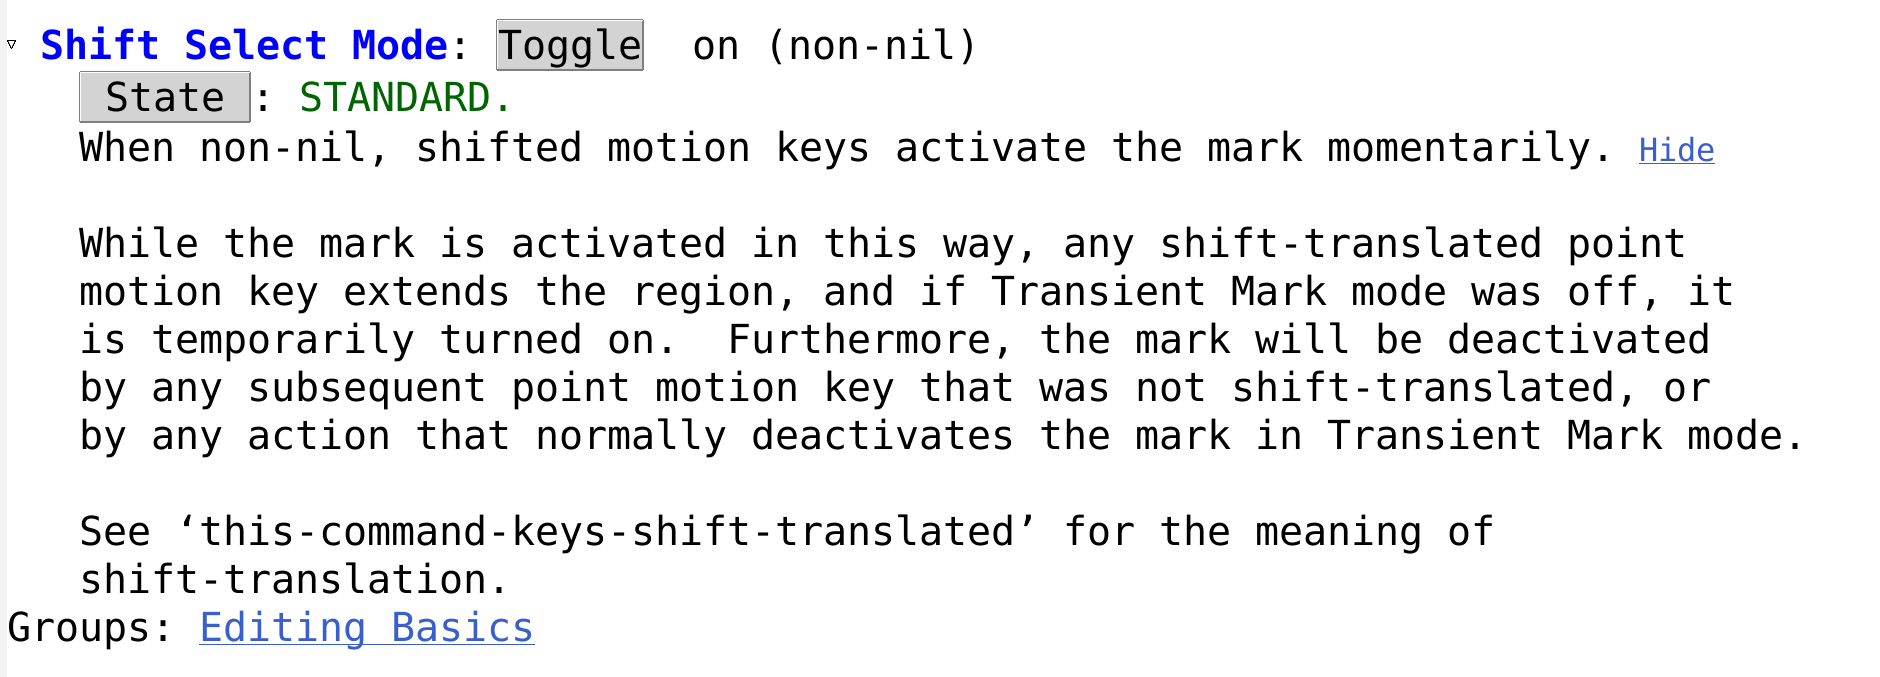
\includegraphics[width=0.8\textwidth]{custom}  
  \caption{Custom user interface}
  \label{fig:custom}
\end{figure}
%
Expecting the user to use \Elisp{} for customization creates a high
barrier.  As a reaction, Per Abrahamsen in 1996 contributed two
libraries called \texttt{Custom} and \texttt{Widget}, which enabled
users to change the values of customization variables via a a UI
rather than through \Elisp{}.  Custom first shipped with Emacs 20.1, XEmacs
20.1 and XEmacs 19.15 (which was released after XEmacs 20.0).
Figure~\ref{fig:custom} shows the UI
for \texttt{shift-select-mode}.

Custom was originally created to customize the Gnus news reader.  With
the integration into both Emacs and XEmacs, Custom also gained an
\Elisp{} programming interface.  The original declaration of
\texttt{shift-select-mode} via the \texttt{defvar} primitive would
have looked like this:
%
\begin{verbatim}
(defvar shift-select-mode t
  "When non-nil, shifted motion keys activate the mark momentarily.
   ...")
\end{verbatim}
%
The Custom library provides the \texttt{defcustom} form, which enables
this declaration:
%
\begin{verbatim}
(defcustom shift-select-mode t
  "When non-nil, shifted motion keys activate the mark momentarily.
   ..."
  :type 'boolean
  :group 'editing-basics)
\end{verbatim}
%
This declaration instantly enables the UI for customizing
\texttt{shift-select-mode}.  The \texttt{:type} declaration as a
boolean makes Custom display a \texttt{Toggle} button.  \Elisp{}
programmers can further gather multiple \texttt{defcustom} variables
into group, creating a hierarchy that Custom also turns into a
navigation API.  The \texttt{:type} declaration can concisely describe
elaborate structures, as in this example:
\begin{verbatim}
(defcustom cc-other-file-alist
  '(("\\.cc\\'"  (".hh" ".h")) ...)
  "Alist of extensions to find given the current file's extension.
..."
  :type '(repeat (list regexp (choice (repeat string) function))))
\end{verbatim}
From this \texttt{:type}, Custom will generate an appropriate UI to
manipulate the value knowing that it is a list of elements, each of which is
a pair of a regular expression and either a list of strings or a function.
This \texttt{:type} can also play the role of documentation.
Custom is now used pervasively in \Elisp{} code, and closely ties the
programming language to the UI.

\subsection{Unicode}
\label{sec:unicode}

As Unicode~\cite{Unicode6} became universally adopted, Emacs and XEmacs both
supported the standard.  Emacs 21.1 added support for the \texttt{utf-8}
coding-system, by adding it as another ``national'' character set.
This meant that an ``é'' coming from a \texttt{utf-8} file was considered a different
character from an ``é'' coming from a \texttt{latin-9} file.  This already
existed before for example between \texttt{latin-1} and \texttt{latin-9} (and many other
character sets), but during the transition to \texttt{utf-8} many more users were
using a mix of two coding systems and were hence affected by this problem.
For this reason, in 2001, Emacs 22.1 introduced a limited form of
unification between character sets.  XEmacs did the same in 2001 with
release 21.4.

As Unicode became a universal text representation and supplanted many
of the earlier encodings, Emacs and XEmacs both started efforts to
replace the internal MULE representation by Unicode altogether.  This
appeared in Emacs 23 (2007) and XEmacs 21.5 (starting about 2010 in a
separate branch).  As a result, the integer representation of a
character in both Emacs and XEmacs is now its Unicode scalar value.

%% FIXME: We should talk about string representations and
%% unibyte-vs-multibyte issues (e.g. whether "\351" should be a string
%% containing the *character* #o351 (i.e. "é") or the string containing the
%% *byte* #o351.

\subsection{Bignums}

Somewhat surprisingly for Lisp, \Elisp{} had no support for
arbitrarily large integers (\emph{bignums}) for many years.
Integer range was restricted by word size on the underlying machine,
and representation changes over time have affected the exact range
available in \Elisp.  (See Section~\ref{sec:data-representation}.)
As a result, various functions dealing with numbers beyond the fixnum range
had to implement workarounds.  Notable are \texttt{file-attributes} (which
may use a pair of two fixnums for inode numbers, device numbers, user id,
and group id, and may use a float for the file size) and
\texttt{current-time}, which returns a list of numbers to encode the time.
Another place where the limited range of integers has caused friction has
been in the fact that it also limits the maximum size of file that can
be edited.

Moreover, \Elisp{} was used for more and more applications beyond
text editing, and also had to implement workarounds.  As a result,
Calc, an advanced calculator and computer algebra tool, which has
shipped with the Emacs distribution since 2001, had to implement
bignum arithmetic in Lisp.

Jerry James added bignums to XEmacs 21.5.18 in 2004, using the GMP
library~\cite{GMP}.  In Emacs, Gerd Möllmann started work on adding support
for bignums via GMP around October 2001, but never finished it.  It was only
in August 2018 that Tom Tromey, with the help of Paul Eggert and several
other developers, finally added support for bignums to Emacs (again, using
GMP).

The support for bignums in XEmacs includes arbitrary-precision integers,
rationals, and floating point numbers and is optional at build time. Thus,
while it is fairly complete, XEmacs's \Elisp{} programs still cannot rely on
bignum support.  Consequently, \texttt{file-attributes},
\texttt{current-time}, and Calc still do not take advantage of bignums.

In contrast, Emacs's bignum support is currently restricted to
arbitrary-precision integers but the feature is provided unconditionally by
bundling the \texttt{mini-gmp} library with Emacs for those systems where
GMP is not installed.  The lack of support for rationals and
arbitrary-precision floats is only a reflection of the lack of interest for
these features.  The support was made unconditional so as to simplify the
system for programmers: the code does
not need to keep alternate code paths for when bignums are not available.
As a result, \texttt{file-attributes} and Calc have been modified to use
native bignums.

Interestingly, bignums in Emacs were always perceived as desirable but never
important enough to overcome the hassle of requiring GMP or some other
multiprecision library.  The deciding factor which changed the tradeoff was probably the fact that by Emacs-25, most builds of Emacs made use of the GNUtls
library (because HTTPS support is more than just desirable), which
internally uses GMP for its cryptography anyway.

The introduction of bignums raises some design issues in \Elisp, as
previously integers were always unboxed.  This meant that the fast
\texttt{eq} only behaved differently from \texttt{eql} on floating point
numbers.  As a result, some \Elisp{} code assumes that if two integers
represent the same number, \texttt{eq} will return true on them.
Bignums are heap-allocated, so the same is not necessarily true for two
bignums.  In XEmacs, \texttt{eq} can return \texttt{nil} in this case, and
this seems to have caused no serious problems.  After a long discussion that
did not reach a consensus, Emacs's maintainers followed XEmacs's design,
because the cost of making \texttt{eq} behave like \texttt{eql} was
considered to be too high, and also because it's a decision that can easily
be changed later without any significant risks of introducing bugs, whereas
the reverse isn't true.

%% ** Major Differences Between 19.11 and 19.12
%% ============================================


%% The new function `type-of' returns a symbol describing the type of a
%% Lisp object (`integer', `string', `symbol', etc.)

%% Symbols beginning with a colon (called "keywords") are treated
%% specially in that they are automatically made self-evaluating when
%% they are interned into `obarray'.  The new function `keywordp' returns
%% whether a symbol begins with a colon.

%% `get', `put', and `remprop' have been generalized to allow you to set
%% and retrieve properties on many different kinds of objects: symbols,
%% strings, faces, glyphs, and extents (for extents, however, this is not
%% yet implemented).  They are joined by a new function `object-plist'
%% that returns all of the properties that have been set on an object.

%% New functions `plists-eq' and `plists-equal' are provided for
%% comparing property lists (a property list is an alternating list
%% of keys and values).

%% The Common Lisp functions `caar', `cadr', `cdar', `cddr', `caaar', etc.
%% (up to four a's and/or d's), `first', `second', `third', etc. (up to
%% `tenth'), `last', `rest', and `endp' have been added, for more
%% convenient manipulation of lists.

%% New function `mapvector' maps over a sequence and returns a vector
%% of the results, analogous to `mapcar'.

%% New functions `rassoc', `remassoc', `remassq', `remrassoc', and
%% `remrassq' are provided for working with alists.

%% New functions `defvaralias', `variable-alias' and `indirect-variable'
%% are provided for creating variable aliases.

%% New macro `push' destructively adds an element to the beginning of a
%% list.  New macro `pop' destructively removes and returns the first
%% element of a list.

%% How did XEmacs bootstrap?
%% Strings with text-properties? No.

\subsection{Terminal-local and frame-local variables, specifiers}

In 1995, Emacs-19.29 added the ability to have \emph{frames} on
several different X11 servers at the same time.  XEmacs evolved
similarly.  This led to a requirement that certain aspects of display
should be local to a frame or an output device.  Emacs calls GUI
windows \emph{frames} and as with buffers, Emacs maintains a reference
to the \emph{current frame} which determines the implicit target of
GUI operations.  XEmacs also maintained \emph{devices} as part of
the display context, to distinguish, say, between different TTYs and
different X11 servers.

As buffer-local variables already allow settings that are sentitive to
context, Emacs furthered the analogy by adding the notion of
\emph{terminal-local} variables, which are variables which take
different values depending on the X11 server (the \emph{terminal}) to
which the current frame belongs.  The set of terminal-local variables
is small and predefined in the C code; they are mostly used internally
to keep track of things like keyboard state; there is no way for
\Elisp{} programs to create others.

XEmacs chose a different route: Starting in 1995, Ben Wing (working
from a prototype by Chuck Thompson) implemented
\emph{specifiers}, which are objects that manage properties that
depend on a generalized notion of \emph{display
  context}~\cite{XEmacsLispRef1998}.  The first prototype
implementation was released with XEmacs 19.12.

A specifier's value (its \emph{instance}) depends on its
\emph{locale}, which can be buffer, a window, a frame, a device, or a MULE
character set, or certain properties of these.

Emacs-20 in 1998 added the ability to set a variable to a frame-local
value.  Contrary to terminal-local variables, any variable can be made
frame-local, and additionally, a variable can be both frame-local and
buffer-local at the same time.

In 2008, during the development of Emacs-23.1 several bugs were found and
fixed in corner case interactions between let-bindings and buffer-local and
frame-local variables (for example, when a variable is made buffer-local
between the moment a let-binding is entered and when it is left), and at
that occasion it was decided that variables should not be allowed to be both
buffer-local and frame-local.

The work on those bugs made it clear that the implementation of buffer-local
and frame-local bindings was too hard to follow, so in 2010 the
implementation was reworked to make the different possible states more
explicit in the code, and at the same time it was decided that frame-local
variables should be deprecated.  Buffer-local variables, however, are used
extensively in \Elisp{} and replacing them with explicit accesses to fields
or properties of buffer objects would make \Elisp{} code heavier.
Frame-local variables were not in widespread use and could easily be
replaced by more traditional use of accessors to frame properties, making it
hard to justify the extra complexity in the implementation.  So in 2012 with
the release of Emacs-24.1, it became impossible to let-bind frame-local
variables any more, and in 2018 with the release of Emacs-26.1, frame-local
variables have been removed altogether.

\section{Post-XEmacs period}           % 2007-now ?
\label{sec:post-xemacs}

Between 1991 and 2001, Emacs improved rather slowly compared to XEmacs.
But starting around 2001, Emacs's pace picked up again.  In 2008 Richard
Stallman stepped down (again) from the maintainership of Emacs, and the new
maintainers have proved more eager to make \Elisp{} evolve, whereas XEmacs
started to lose momentum starting about 2010.
%% Sadly, many improvements in XEmacs have never been
%% incorporated back into Emacs.

This section discusses some notable evolution of the design of
\Elisp{} after 2010 which have not found their way into XEmacs so far.

\subsection{Lexical scoping}
\label{sec:lexical-scoping}

When Richard Stallman started working on \Elisp, lexical scoping
was becoming the established standard in the Lisp family in both
Common Lisp and Scheme.  So of course, the question of adding lexical
scoping to \Elisp{} has been brought up many times.

The first implementation appeared quite early, in the form of the
\texttt{lexical-let} macro, which was part of the new \texttt{cl.el} by Dave
Gillespie \email{<daveg@synaptics.com>} introduced in 1993 and which
performed a local form of closure-conversion.
While this macro was used in many packages, it was never considered as
a good solution to the problem of providing lexical scoping.
The somewhat long name was likely a factor, but the reason was more probably
due to the fact that the code generated by the macro was less efficient than
equivalent dynamically-scoped code and was more difficult to debug because
the backtrace-based debugger showed you the gory details of the
macro-expansion rather than the corresponding source.  For these reasons,
\texttt{lexical-let} was only used in those particular cases where lexical
scoping was really beneficial.

Dynamic scoping had two main drawbacks in practice:
\begin{itemize}
\item \textit{The lack of closures.}
  Some packages circumvented the lack of closures
  by building lambda expressions on the fly with constructs like
  \verb|`(lambda (x) (+ x ',y))|, which suffered from various problems
  such as the fact that macros within that closure were expanded late, and
  its code was not seen by the byte-compiler.  Emacs-23.1 introduced the
  curry operator \texttt{apply-partially} to cover similar use cases without
  those drawbacks.  In all cases, the programmer had to manually specify
  which variables to capture from the environment, with very little help
  from the tools to detect errors in this respect.
\item \textit{The global visibility of variable names,} requiring more care with the
  choice of local names.  The convention followed in Emacs to name all
  global variables with a package-specific prefix works well to avoid name
  conflicts: it not only avoids conflicts between global variables, but also
  between local variable and global variables since local variables do not
  have such a prefix.  The only remaining possible conflicts occur between
  local variables of different functions.  In Elisp these tend to happen only
  in the presence of higher-order functions.  For example in code such as:
\begin{verbatim}
    (let ((lst (some-list)))
      (cl-every (lambda (x) (memq x lst)) elements))
\end{verbatim}
  where a variable capture occurs if \texttt{cl-every} happens to bind a local
  variable \texttt{lst} before calling its first argument.  Name conflicts
  were also problematic in one other special case, the byte-compiler: in
  order to emit warnings about the use of undeclared variables, the
  byte-compiler just tested whether that variable was already known to
  Emacs, which always returned true for those variables locally bound by one
  of the functions on the call stack, such as the functions in the
  byte-compiler itself.  So some code in the byte-compiler was made uglier
  with long local variable names in order not to interfere with other local
  bindings.  Worse: these ``solutions'' were never really complete.
\end{itemize}
%%
The only fully satisfactory solution to the desire for lexical scoping in
\Elisp{} was that it should be the scoping used by default by all binding
constructs, with an easy way to request dynamic scoping for some
variables, as is the case in Common Lisp.  But at the same time, there was
a non-negotiable need to preserve compatibility with existing \Elisp{} code,
although some limited breakage for rare situations could be tolerated.

The vast majority of existing \Elisp{} code was (and still is) agnostic to
the kind of scoping used in the sense that either dynamic or lexical scoping
of local variables gives the same result in almost all circumstances.  This was true of early
\Elisp{} code and has become even more true over time as the byte-compiler
started to warn about references to undeclared variables.  Warnings about
unused variables would have probably pushed even more \Elisp{} code to be
agnostic.  But in any case, it seemed clear that despite the above, the
majority of Elisp packages relied somewhere on dynamic scoping.  So while
there was hope to be able to switch \Elisp{} to use lexical scoping, it was
not clear how to find the few places where dynamic scoping is needed so as
to avoid breaking too many existing packages.

In 2001, Matthias Neubauer implemented a code
analysis that, instead of trying to find the places where dynamic scoping is
needed, tries to find those bindings for which lexical scoping would not
change the resulting semantics~\cite{Neubauer01}.
This tool could have been used to
mechanically convert \Elisp{} packages to a lexically scoped version of
\Elisp{}, while preserving the semantics.  The plan with this approach
was to facilitate moving \Elisp{} code to Scheme eventually, but the
overall project was too large to ever be realized.

In late 2001, Miles Bader started working on a branch of Emacs called
\emph{lexbind} with support for lexical scoping, which was finally included
in Emacs-24.1.  The solution he adopted was to have two languages: an
\Elisp{} with dynamic scope for backward compatibility, and another with
scoping rules like those of Common Lisp, i.e.~lexical scope by default
except for those variables that have been declared as dynamically scoped (in
practice, these are all the global variables).  Each file is tagged to
indicate which language is to be used (defaulting to the backward compatible
mode), and in turn, each function value is tagged with the language it is
using, so functions using dynamic scope can seamlessly call functions with
lexical scope and vice versa.  This way, old code keeps working exactly
as before and any new code that wants to benefit from lexical scoping
simply has to add the corresponding ``\texttt{-*- lexical-binding:t -*-}''
annotation at the beginning of the file.

The two languages were sufficiently similar that the new lexically scoped
variant only required minor changes to the existing interpreter.  But the
changes needed to support this new language in the byte-compiler were more
problematic, causing progress on this branch to be slow.  This branch was
kept up-to-date with the main Emacs development but the modifications to the
byte-compiler were never completed.

%% https://lists.gnu.org/r/emacs-devel/2001-10/msg00560.html
Finally in 2010 Igor Kuzmin worked on a summer project under the direction
of Stefan Monnier, in which he tried to add lexical scoping to the
byte-compiler differently:
instead of directly adding support for lexical scoping and closures to the
single-pass byte-compiler code (which required significant changes to the
code and was made more complex by the need to fit into a single pass), he
implemented a separate pass (itself split into two passes) to perform
a traditional closure conversion as a pre-processing step.  This freed the
closure conversion from the constraints imposed by the design of the
single-pass byte-compiler, making it much easier to implement, and it also
significantly reduced the amount of changes needed in the byte-compiler,
thus reducing the risk of introducing regressions.

Two years later, Emacs-24.1 was released with support for lexical
scoping based on Miles Bader's \emph{lexbind} branch combined with Igor's
closure conversion.  The main focus at that point was to:
\begin{itemize}
\item minimize the changes to the existing code to limit incompatibility
  with existing \Elisp{} packages;
\item make sure performance of existing code was not measurably affected by
  the new feature;
\item provide reliable support for the new lexical scoping mode, though not
  necessarily with the best performance.
\end{itemize}
%%
Changes to the byte code were introduced as part of the lexical scoping
feature that appeared in 2012 in Emacs-24.1, but were actually developed
much earlier, probably around 2003: until the introduction of
lexical-scoping, the stack-based byte-code only used its stack in the most
simple way, and did not include any stack operation beyond
\texttt{pop}/\texttt{dup}/\texttt{exch}, so to better support lexical
scoping where the lexical variables are stored on the stack, several
byte-codes were added to index directly into the stack, to modify stack
slots, and to discard several stack elements at once.

Performance of the new lexical scoping mode proved to be competitive with
the performance of the dynamic scoping mode except for its interaction with
the \texttt{catch}, \texttt{condition-case}, and \texttt{unwind-protect}
primitives whose underlying byte-codes were a poor fit, requiring run-time
construction of \Elisp{} code to propagate the lexical context into the body
of those constructs.
So in Emacs-24.4, new byte codes were introduced and
the byte-code compiler was modified to be able to make use of them.  Nowadays,
code compiled using lexical scoping is generally expected to be marginally
faster than if compiled with dynamic scoping.

The introduction of \texttt{lexical-binding} in Emacs-24.1 went very smoothly,
causing only few backward incompatible changes for users, in part because
very few of Emacs's own files made use of it.  Converting existing code to
use the new language is usually easy (consisting mainly in adding a few
variable declarations, with the help of warnings from the byte-compiler) but
is not automated and can sometimes require a non-trivial effort for packages
which make heavy or creative use of dynamic scoping.  Nowadays, most new
packages choose to use the new lexically scoped language, and about half the
well-maintained packages have converted to it, but there is still a large
amount of code using the old language, either because they still want to
support Emacsen older than Emacs-24.1, or because of the effort needed to
convert.  For example, as of Emacs-26, only a third of Emacs's own Lisp code
has been converted to use lexical scoping.


\subsection{Eager macro-expansion} %Emacs-24.3?
\label{sec:eager-macro-expansion}

The exact time at which a macro is expanded has never been clearly specified
in \Elisp{}.  Until Emacs-24, macro-expansion usually took place as late as
possible for interpreted code, whereas for byte-compiled code,
macro-expansion always took place during byte-compilation, with some notable
exceptions where the code was ``hidden'' from the byte-code compiler.  In the
byte-code compiler, the macro-expansion was also done ``lazily'' in that it was
done on the fly during the single pass of compilation.

In order to implement the separate closure conversion phase for Emacs-24,
this had to be changed so that the code is macro-expanded in a separate
phase before closure conversion and the actual byte-compilation, using a new
\texttt{macroexpand-all} function.
This caused some visible differences in corner cases where some macro
invocations were expanded which earlier had been eliminated by optimizations before
getting to the point of macro-expansion. In practice, this did not cause
any serious regression.

This use of the new \texttt{macroexpand-all} function was made yet a bit
more prevalent in Emacs-24.3 which applies it when loading
a non-compiled file, so that macro-expansion now happens ``eagerly'' when
loading a file rather than lazily when Emacs actually runs the code.  This eager
macro-expansion occasionally bumps into problematic dependencies (typically
in files which were never compiled), so it fails gracefully: if an
error is signaled during the macro-expansion that takes place while loading
a file, Emacs just aborts the macro-expansion and continues with the non-expanded
code as in the past, though not without duly notifying the user about
the problem.

Emacs-25.1 additionally fine-tuned these macro-expansion phases (both
while loading a file and while compiling them) according to the section
3.2.3.1 of the Common Lisp HyperSpec~\cite{HyperSpec}, so as to improve the
handling of macros that expand to both definitions and uses of
those definitions.

\subsection{Pattern matching}           %Released in Emacs-24.1
\label{sec:pcase}

While working on the \texttt{lexical-binding} feature, Stefan Monnier grew
increasingly frustrated with the shape of the code used to traverse the
abstract syntax tree, littered with \texttt{car}, \texttt{cdr} carrying too
little information, compared to the kind of code he would write for that in
statically-typed functional languages with algebraic datatypes.

So he started working on a pattern matching construct inspired by those
languages.  Before embarking on this project, he looked for existing
libraries providing this kind of functionality, finding many of them for
Common Lisp and Scheme, but none of them satisfying his expectations: either
the generated code was not considered efficient enough, or the code seemed
too difficult to port to \Elisp{}, or the set of accepted patterns was too
limited and not easily extensible.

So the \texttt{pcase.el} package was born,
first released as part of Emacs-24.1, and used extensively in the part
of the byte-code compiler providing support for lexical scoping.

Additionally to the \texttt{pcase} macro itself that provides a superset of
Common Lisp's \texttt{case} macro, this package also provides the
\texttt{pcase-let} macro, which uses the same machinery and supports the same
patterns in order to deconstruct objects, but where it is allowed to assume
that the pattern does match and hence can skip all the tests, leaving only the
operations that extract data.

After the release of Emacs-24.1, Stefan was made aware of Racket's
\texttt{match} construct~\cite{RacketReference2018}, which had somehow eluded
his earlier search for
existing pattern matching macros and whose design makes it easy to define
new patterns.  The implementation of Racket's \texttt{match} could not be
easily reused in \Elisp{} because it relies too much on the compiler's
efficient handling of locally defined functions, but \texttt{pcase.el} was
improved to follow some of the design of Racket's \texttt{match}.
The new version appeared in Emacs-25.1 and the main resulting novelty was the
introduction of \texttt{pcase-defmacro} which can define new patterns
in a modular way. %% often using the new low-level pattern \texttt{app}.

\subsection{CL-lib}          %Released in Emacs-24.3
\label{sec:cl-lib}

While the core of \Elisp{} has evolved very slowly over the years, the
evolution of other Lisps (mostly Scheme and Common Lisp) put pressure to
try and add various extensions to the language.  As it turns out, \Elisp{},
to a first approximation, can be seen as a subset of Common Lisp, so by
1986 Cesar Quiroz \email{<quiroz@cs.rochester.edu>} had already written
a \texttt{cl.el} package that provided various
Common Lisp facilities implemented as macros.  Emacs 18.51 was the
first Emacs release to ship with \texttt{cl.el}, in 1988.  It was superceded
5 years later for Emacs-19.18 by a new version contributed by Dave
Gillespie with a more detailed emulation of Common Lisp as well as a few
extensions.

Richard Stallman never wanted \Elisp{} to morph into Common Lisp, but he saw
the value of offering such facilities, so this \texttt{cl.el} package was
included with Emacs fairly early, and has been one of the most popular
packages, used by a large proportion of \Elisp{} packages.  Yet,
Stallman did
not want to impose \texttt{cl.el} onto any Emacs user, so he imposed
a policy where the use of \texttt{cl.el} was restricted \emph{within} Emacs
itself.  More specifically, \Elisp{} packages bundled with Emacs were
restricted to limit their use of \texttt{cl.el} in such a way that
\texttt{cl.el} never needed to be loaded during a normal editing session.
Concretely, this meant that the only features of \texttt{cl.el} that could
be used were macros and inlined functions.

The reasons why Stallman did not want to use \texttt{cl.el} and turn \Elisp{}
into Common Lisp are not completely clear, but the following elements seem
to have been part of the motivations:
\begin{enumerate}
\item Common Lisp was considered a very large language back then, so in all
  likelihood it would have taken a significant effort to really make
  \Elisp{} into a reasonably complete implementation of Common Lisp.
\item Some aspects of Common Lisp's design can incur 
  significant overhead, and Emacs already carried the stigma of being
  too big.  (\texttt{vi} advocates used the derogatory epithet \emph{eight
  megabytes and
    constantly swapping} in the days when eight megabytes were a
  significant amount of memory.)  Consequently, there were good reasons to avoid making
  \Elisp{}'s efficiency any worse.
\item Many aspects of Common Lisp design were decided by majority not consensus, as
  evidenced by the divide between Common Lisp and Scheme.
  Stallman disliked several aspects of Common Lisp's design, such as the use of
  keyword arguments, especially in low-level primitives like
  \texttt{mapcar}~\cite{RMS-keyword-args-are-clunky}.
\item Keeping \Elisp{} small meant that users could participate in its
  development without having to learn all of Common Lisp.  When inclusion of
  Common Lisp features was discussed, Stallman would often point out the cost
  in terms of the need for more, and more complex,
  documentation~\cite{RMS-cl-big-doc}.
\item The implementation of \texttt{cl.el} was fairly invasive, redefining
  some core \Elisp{} functions.
\item Finally, turning \Elisp{} into Common Lisp would imply a loss of control,
  in that Emacs would be somewhat bound to Common Lisp's evolution and would
  have to follow the decisions of the designers of Common Lisp on most aspects.
\end{enumerate}
Over the years, the importance of the first two points has waned to some
extent.  Also the popularity of the \texttt{cl.el} package, as well as the
relentless pressure from Emacs contributors asking for more Common Lisp
features has also reduced the relevance of the fourth point.

XEmacs took the easy route on this and loaded \texttt{cl.el} into the
standard XEmacs image, starting with XEmacs 19.14 in 1996.  Emacs instead
took a longer road, where over the years, various macros and functions from
\texttt{cl.el} were found to be sufficiently clean and popular to justify
moving them into \Elisp{} proper:

\begin{itemize}
\item[1997] The release of Emacs-20.1 saw the move of the
  macros \texttt{when} and \texttt{unless} as well as the functions
  \texttt{caar}, \texttt{cadr}, \texttt{cdar}, and \texttt{cddr}.
\item[2001] Then maintainer Gerd Möllmann had a more favorable opinion of
  Common Lisp.  As a result, Emacs-21.1 included the hash-table functions,
  reimplemented in C and extended.  It also adopted the Common Lisp concept
  of \emph{keyword} symbols, to ease the work of \texttt{cl.el} as well as
  for the benefit of other packages making use of them.  Additionally, the
  macros \texttt{dolist}, \texttt{dotimes}, \texttt{push}, and \texttt{pop}
  were also added to \Elisp{}, although they introduced some difficulties: in
  \texttt{cl.el} those macros included extra functionality, which relied on
  parts of \texttt{cl.el} which were not needed in core \Elisp, specifically
  \texttt{block}/\texttt{return} and generalized variables.  For that reason
  the macros added to \Elisp{} did not actually replace those of
  \texttt{cl.el}; instead when \texttt{cl.el} was loaded, it overrode the
  original macros with its own version.
\item[2007] Emacs-22.1 added \texttt{delete-dups}, which provided a subset of
  \texttt{cl.el}'s \texttt{delete-duplicates}.
\item[2012] Emacs-24.1 added \texttt{macroexpand-all} and lexical scoping,
  which obsoleted \texttt{cl.el}'s \texttt{lexical-let}.
\item[2013] Emacs-24.3 added compiler macros, \texttt{setf} and
  generalized variables.
\item[2018] To the \texttt{cXXr} functions incorporated in Emacs-20.1,
  Emacs-26.1 added the remaining \texttt{cXXXr} functions.  The resistance
  against those was mostly one of style, since they tend to lead to code
  that is difficult to read.
\end{itemize}
The details here are not terribly important, but rather the fact that there
has been a regular trickle of features seeping out of \texttt{cl.el} into
\Elisp{}, and that in many if not most cases this took place not by just
moving code from \texttt{cl.el} but by reimplementing it, often with
slightly different semantics.

During the development of Emacs-24.3 the issue of better integration of the
\texttt{cl.el} package came up again.  The main point of pressure was the
desire to use \texttt{cl.el} \emph{functions} within packages bundled with
Emacs.  Richard Stallman still opposed it, but this time, a compromise was
found: replace the \texttt{cl.el} package with a new package
\texttt{cl-lib.el} that provides the same facilities, but with names that
all use the \texttt{cl-} prefix.  This way, the \texttt{cl-lib.el} package
doesn't turn \Elisp{} into Common Lisp, but instead provides Common Lisp
facilities under its own namespace, leaving \Elisp{} free to evolve in its
own way~\cite{RMS-cl-real}.

The implementation of \texttt{cl-lib} mostly just took \texttt{cl.el} and
added the \texttt{cl-} prefix to its definitions while at the same time
a new \texttt{cl.el} was implemented which is just a very thin wrapper
re-exporting the \texttt{cl-lib} definitions under their old names.  Yet,
some details of \texttt{cl.el}'s implementation were also reworked to be
less invasive.  The main aspect was that \texttt{cl.el} redefined Emacs's
macro-expansion wholesale with its own implementation, which incorporated
support for compiler macros, \texttt{lexical-let}, \texttt{flet}, and
\texttt{symbol-macrolet}, so this was reworked by extending the standard
macro-expansion code so \texttt{cl-lib.el} could provide those features
more cleanly.

To encourage adoption of this new library, a forward compatibility version
of \texttt{cl-lib.el} for use on older Emacs and XEmacs versions was
released at the same time as Emacs-24.3.  Despite the annoyance of having to
use a \texttt{cl-} prefix, which caused some resistance to this new library,
the change has been surprisingly successful if we look at the proportion of
new packages which use \texttt{cl-lib.el} instead of \texttt{cl.el}.

Nowadays, both \texttt{cl-lib.el} and \texttt{cl.el} are bundled with Emacs
and supported, but \texttt{cl.el} is not used by Emacs's own Lisp code any
more, and it is expected to be declared obsolete in Emacs-27.
But it's been very popular for many years, so it will take a long time
before we can really retire it.  And this thin wrapper is sufficiently
simple that it doesn't incur much cost either in terms of maintenance
or performance.

\subsection{Generalized variables} %Released in Emacs-24.3
\label{sec:generalized-variables}

To facilitate the move to \texttt{cl-lib.el}, some frequently used
functionality from \texttt{cl.el} was moved directly to \Elisp{}.  The most
visible one is the support for \emph{generalized variables}, also variously
known as \emph{places}, \emph{generalized references}, or \emph{lvalues}.
A generalized variable is a form that can be used both as an expression and
as an updateable reference.  The concept comes from Common Lisp, and the
Emacs implementation originally a part of \texttt{cl.el}.  In both Common
Lisp and Emacs, a number of special forms take generalized variables as
operands---in particular, \texttt{(setf \id{PLACE} \id{VALUE})}, which treats
a generalized variable as a reference and sets its value.

In Common Lisp, macros can invoke \texttt{get-setf-expansion}
to turn a place into a list of five elements:
\begin{displaymath}
  (\id{VARS}~\id{VALS}~\id{STORE-VAR}~\id{STORE-FORM}
  ~\id{ACCESS-FORM})
\end{displaymath}
where \id{VARS} and \id{VALS} together form a list of bindings which perform
the computation needed to reach the place and should be done only once
(for reasons of performance or side-effects); \id{ACCESS-FORM} lets you then
read the current value of the place; and \id{STORE-VAR} and \id{STORE-FORM}
specify how to \emph{set} the place (by binding \id{STORE-VAR} to the
desired value and then executing \id{STORE-FORM}).

For example the macro \texttt{(push \id{EXP} \id{PLACE})}, which adds
\id{EXP} to the head of the list stored in \id{PLACE}, could be defined to
expand to:
%
\begin{center}
\texttt{(setf \id{PLACE} (cons \id{EXP} \id{PLACE}))}
\end{center}
%
But that would duplicate \id{PLACE} which could perform a costly operation
and have side-effects.  So the macro instead uses
``\texttt{get-setf-expansion}'' in order to expand to code of the following
form:
\begin{displaymath}
  \MAlign{
    \texttt{(let ((v \id{EXP}))} \\
    \;\;\;\MAlign{
      \texttt{(let* (\id{VARS} = \id{VALS})} \\
      \;\;\;\MAlign{
        \texttt{(let ((\id{STORE-VAR} (cons v \id{ACCESS-FORM})))} \\
        \;\;\;\id{STORE-FORM}))}}}
\end{displaymath}
This imposes a fairly rigid structure which, while general enough to adapt
to most needs, can be burdensome and leads to verbose code with a lot
of plumbing, both in the implementation of places and in the implementation
of macros which take places as arguments.

The original \texttt{cl.el} code followed this Common Lisp design.  But when
implementing the support for \texttt{setf} and friends in \Elisp{}, a fresh
new implementation of the concept was used.  The reasons for this new
implementation were:
\begin{itemize}
\item The implementor of \texttt{cl-lib} (Stefan Monnier) found the existing
  code was hard to follow, arguably a case of
  ``not-invented-here syndrome'' on Stefan's part.
\item The previous code made use of internal helper functions from
  \texttt{cl.el} which the maintainers did not want to move to core \Elisp,
  so some significant massaging was needed anyway.
\item Stefan Monnier considered this part of Common Lisp's
  design ugly.
\end{itemize}
%% For example, if we want to define a place
%% of the form $\texttt{(if~\textsl{TEST}~\textsl{PLACE1}~\textsl{PLACE2})}$
%% the above \texttt{push} will inevitably end up with one of two
%% possibilities:
%% \begin{itemize}
%% \item Check twice whether \textsl{TEST} was nil or not: once within
%%   \textsl{ACCESS-FORM} and once within \textsl{STORE-FORM}.
%% \item Do the check once within \textsl{VALS} to return a pair of an ``access
%%   function'' and a ``store function'' which are then called via
%%   \texttt{funcall} within \textsl{ACCESS-FORM} and \textsl{STORE-FORM}.
%% \end{itemize}
%%
So the reimplementation uses a different design: instead of a five element
list, the new function \texttt{gv-get-place-function} turns
a \emph{place}  into a single higher-order function.
This higher-order function takes as its sole argument a function
of two arguments (the \textsl{ACCESS-FORM} and the \textsl{STORE-FUNCTION})
which should return the code that we want to perform on the place.
For example, the \texttt{push} macro could be implemented as:
\begin{verbatim}
    (defmacro push (EXP PLACE)
      `(let ((x ,EXP))
         ,(funcall (gv-get-place-function PLACE)
                   (lambda (ACCESS-FORM STORE-FUNCTION)
                     (funcall STORE-FUNCTION `(cons x ,ACCESS-FORM))))))
\end{verbatim}
%% and this can be streamlined a bit with the use of the macro
%% \texttt{gv-letplace} which lets us write the above as:
%% \begin{verbatim}
%%     (defmacro push (EXP PLACE)
%%       `(let ((x ,EXP))
%%          ,(gv-letplace (ACCESS-FORM STORE-FUNCTION) PLACE
%%             (funcall STORE-FUNCTION `(cons x ,ACCESS-FORM)))))
%% \end{verbatim}
This design generally leads to cleaner and simpler code, and we can easily
provide backward compatibility wrappers for most of Common Lisp's
primitives.

A Common-Lisp-style representation of a place can easily be turned into
its corresponding higher-order function.  The reverse is not true, however, so
this design precludes compatibility with Common Lisp and
\texttt{cl.el}'s \texttt{get-setf-expansion}, which must produce the
five values described above.
Breaking compatibility with \texttt{get-setf-expansion}
was of course
a downside, but in practice this function was almost never used outside of
\texttt{cl.el} itself so very few packages were impacted by
this incompatibility.

\subsection{Object-oriented programming} %Emacs-25.1
\label{sec:oop}

While \texttt{cl.el} provided compatibility with Common
Lisp's \texttt{defstruct} early on (Section~\ref{sec:structures}), including the
ability to define new structs as extensions/subtypes of others, thus
providing a limited form of inheritance, actual support for object-oriented
programming in the form of method dispatch has been historically limited
in Emacs.

The first real step in that direction was the development of EIEIO by Eric
Ludlam around the end of 1995, beginning of 1996.  The official name ``Enhanced
Implementation of Emacs Interpreted Objects'' hints at the earlier existence
of some ``Emacs Interpreted Objects'' package but in reality the acronym
came before its expansion was chosen, because of the comic reference to the
nursery rhyme.
EIEIO started as an experiment to try to use
an object system in Emacs, first following a model like that of C++, but
very soon switching to a CLOS-inspired model.

\subsubsection{CLOS}

EIEIO is an implementation of a subset of CLOS, the Common Lisp Object
System~\cite{DeMichielGabriel1987}.  CLOS is a somewhat unusual object
system where methods are not attached to objects or classes; instead, it
provides the notion of \emph{generic function} which are functions
implemented by a set of methods where each method indicates when it is
applicable by annotating its arguments with a \emph{specializer} which is
usually a type indicating that this method is applicable only if this
argument belongs to this type.  This type-based dispatch is not limited to
the first argument but can be applied to any number of arguments, a feature
called \emph{multiple-dispatch}.  Furthermore, when several methods can be
applied, the programmer can control how the methods are \emph{combined}, for
example by adding \emph{qualifiers} (like \texttt{:after}, or
\texttt{:before}).  Beside generic functions, CLOS also provides the
\texttt{defclass} macro to define new types by listing their parents,
fields, and various other properties.

Here is an example of CLOS code which defines a new \texttt{point3d} subclass
of a pre-existing \texttt{point2d} class, and add a new method to the
generic function \texttt{point-distance}, but only when both
arguments are subtypes of \texttt{point3d}:
\begin{verbatim}
    (defclass point3d (point2d)
      (z :documentation "Third dimension"))
    (defmethod point-distance ((p1 point3d) (p2 point3d))
      (let ((distance2d (call-next-method))
            (distancez (- (slot-value p1 'z) (slot-value p2 'z))))
        (sqrt (+ (* distance2d distance2d)
                 (* distancez distancez)))))
\end{verbatim}

\subsubsection{EIEIO}

Just like \Elisp{}, the development of EIEIO was mostly
driven by actual needs more than as an end in itself: the original
motivation was to try and play with an object request broker, then a widget
toolkit, and later switched to providing support for the CEDET
package, a package providing IDE-like features~\cite{Ludlam18}.
It included support for most of CLOS's \texttt{defclass}, as well as support
for a subset of \texttt{defmethod}, more specifically it was limited to
single-dispatch methods, dispatching on the first argument, and it could
only dispatch based on types of \texttt{defclass} objects.  It also had
incomplete support for method combinations, only allowing \texttt{:before}
and \texttt{:after} methods but not \texttt{:around} nor any user-defined
additional qualifiers.

EIEIO spent most of its life as part of the CEDET package
before being integrated into Emacs-23.2 in
2010, along with most of CEDET.  Use of EIEIO within Emacs stayed fairly
limited, partly for reasons of inertia, but also because EIEIO suffered some
of the same problems as \texttt{cl.el} in that it was not
``namespace clean''.

\subsubsection{CL-generic}

At the end of 2014, Stefan Monnier started to try and clean up EIEIO so as
to be able to use it in more parts of Emacs.  The intention was basically to
add a ``\texttt{cl-}'' prefix as was done for \texttt{cl-lib} (because it
was perceived that an ``\texttt{eieio-}'' prefix would be too verbose to be
popular), but there was also a desire to improve the \texttt{defmethod} with
support for \texttt{:around} methods and dispatch on other types than those
defined with \texttt{defclass}.

It became quickly evident that the implementation of method dispatch
needed a complete overhaul: rather than constructing combined methods
up-front and memoizing the result, as in typical CLOS implementations,
EIEIO's dispatch and \texttt{call-next-method} did all their work
dynamically, relying on global variables to preserve state in
a way that was both brittle and somewhat inefficient.

So, instead of improving EIEIO's \texttt{defmethod}, a completely new
version of CLOS's \texttt{defmethod} was implemented in the new
\texttt{cl-generic.el} package, which appeared in Emacs-25.1.  The main
immediate downside was that the idea to cleanup the rest of EIEIO (which
implements \texttt{defclass} objects) ended up forgotten along the way.
The implementation is not super efficient, but it's already several times
faster than the previous one in EIEIO.  This package provides largely the
same featureset as CLOS's \texttt{defmethod}, except for some important
differences:
\begin{enumerate}
\item Method combinations cannot be specified per method like in CLOS, but
  instead new method combinations can be added globally by adding
  appropriate methods to
  \texttt{cl-\linebreak[0]generic-\linebreak[0]combine-\linebreak[0]methods}.
  This seemed like a good idea, but there is no known user of this feature
  at this time, not even internal.
\item The set of supported specializers is not hard-coded.  In CLOS,
  a specializer can be either a type (indicating the this method applies when the argument is of
  this type) or of the form \texttt{(eql \id{VAL})}, indicating that the
  method only applies when the argument is equal to \id{VAL}.
  \Elisp{} extends this so new specializers
  can be defined in a modular way via the notion of \emph{generalizer}
  inspired from~\citet{Rhodes14}.  This is used both internally (to define
  all the standard specializers) as well as in some external packages, most
  notably in EIEIO to support dispatching on \texttt{defclass} types.
\end{enumerate}
The main motivation for the first difference above was that CLOS's support
for method combinations seemed too complex: the cost of implementation was
not justified by the expected use of the feature, so it was replaced by
a much simpler mechanism.

As for the second difference, it was made necessary by the need to dispatch
on EIEIO objects even though \texttt{cl-generic.el} could not depend on
EIEIO since it was not clean enough.  There were additional motivations for
it, though: not only was it clearly desirable to be able to define new
specializers, but it also made the implementation of the main specializers
cleaner, and most importantly it seemed like an interesting problem
to solve.

Some existing \Elisp{} functions appeared like good candidates to use that
machinery to split them into independent methods but required dispatching
on contextual information (i.e.\ on the current state) rather than only on
arguments.  Consequently, \texttt{cl-generic.el} also adds support to its
\texttt{cl-defmethod} for pseudo-arguments of the form ``\texttt{\&context
  (\id{EXP} \id{SPECIALIZER})}'' which means that this method is
applicable when \id{EXP} evaluates to a value that satisfies the
\id{SPECIALIZER} constraint.  This is used for methods which
are only applicable in specific contexts, such as in specific major modes or
in frames using a particular kind of GUI.

\subsubsection{Overall support for classes}

The implementation of \texttt{cl-generic.el} was accompanied by an extension
of the on-line help system so as to be able to give information not just
about \Elisp{} variables, functions, and faces but also other kinds of named
elements, starting with types.  And to go along with that, the implementation
of \texttt{cl-defstruct} was improved to better preserve information about
the type hierarchy so that the on-line help system can be used to browse
it.  This started as an attempt to adapt to \texttt{cl-generic.el} the EIEIO
facilities to interactively explore EIEIO objects and methods, but is more
modular and better integrated with the rest of Emacs's on-line help system.

As of Emacs-26, object support in \Elisp{} is hence split into four parts: the
old \texttt{cl-defstruct} provided by \texttt{cl-lib.el} which allows
defining new object types and supports single-inheritance; \texttt{defclass}
provided by EIEIO which offers similar functionality plus multiple
inheritance and a few other benefits but at the cost of slower object
creation and field accesses; \texttt{cl-defmethod} provided by
\texttt{cl-generic.el} which allows defining methods and supports
\texttt{cl-defstruct} objects and \texttt{defclass} objects equally; and finally
\texttt{defmethod} which is the deprecated method definition of EIEIO which
has been reimplemented as a wrapper on top of the new \texttt{cl-defmethod}
(this backward compatibility library is deprecated and a bit less efficient
than using \texttt{cl-defmethod} directly but still more efficient than its
earlier implementation, and it is fully implemented using documented features
of \texttt{cl-defmethod}, so it doesn't impose any performance or
maintenance issue).  Emacs will likely live with both \texttt{cl-defstruct} and
\texttt{defclass} for the foreseeable future.

\subsection{Actual objects}  %Emacs-26.1
\label{sec:actual-objects}

While Emacs-25's \texttt{cl-generic.el} introduced object-oriented
programming facilities into \Elisp{}, objects (whether defined via
\texttt{cl-lib}'s \texttt{cl-defstruct} or EIEIO's \texttt{defclass}) were
still represented as vectors and hence couldn't be reliably distinguished
from vectors, for example to pretty-print them.

This was addressed in Emacs-26 by the introduction of the
\texttt{make-record} primitive and corresponding new object type.
(See also Section~\ref{sec:structures}.)
Those \emph{records} are implemented just like the vectors used previously,
except that their tag indicates that they should be treated as records
instead of vectors, and that by convention the first field of a record is
supposed to contain a type descriptor, which can be just a \emph{symbol}.

The main complexity introduced by this change was the need for a new syntax
to print and read those new objects, as well as the incompatibility between
the printed representation of objects using the old vector-based encoding
and those using the new encoding.

\subsection{Generators}
\label{sec:generators}

With the success of Python's and Javascript's iterators and generators, some
Emacs users felt like \Elisp{} was lacking in abstraction, so in 2015,
Daniel Colascione developed \texttt{generator.el}, which was included
into Emacs-25.1.  It makes it easy and convenient to write generators using
macros \texttt{iter-lambda} and \texttt{iter-yield}.  Its implementation is
based on a kind of local conversion to continuation-passing style (CPS) and
hence relies extensively on the use of lexical scoping, to work around the
fact that \Elisp{} does not directly provide something like \texttt{call/cc}
to access underlying continuations.  It only handles a (relatively large)
subset of \Elisp{}, because CPS conversion of forms like
\texttt{unwind-protect}~\cite{HaynesFriedman1987} cannot be defined in general in \Elisp.

\subsection{Concurrency}
\label{sec:concurrency}

\Elisp{} is a fundamentally sequential language, and it relies very heavily
on side-effects to a global state.  Yet, its use in an interactive program
has inevitably lead to a desire for concurrency to try and improve
responsiveness.  Concurrency appeared very early on: since
Emacs-16.56, Emacs has included support for asynchronous processes, i.e.~the
execution of separate programs whose output was processed by so-called
\emph{process filters} whenever the \Elisp{} execution engine is idly
waiting for the next user input.

While this very limited form of cooperative concurrency was slightly
improved in 1994's Lucid Emacs 19.9 and 1996's Emacs-19.31 by adding native support for timers (they
had earlier been implemented as an asynchronous process sending Emacs output at
the requested time), it has been the only form of concurrency available for
most of Emacs's life.

Adding true shared-memory concurrency to \Elisp{} is problematic because of
the pervasive reliance on shared state in existing \Elisp{} code.  In some
cases, shared state is not a problem and concurrency can be mimicked via
asynchronous programming: When a program waits for an operation (such as an
external program), instead of blocking, it registers a continuation callback
and returns control to the main event loop.  Yet many \Elisp{} packages
instead block, because slicing the execution via callback means effectively
writing code in continuation-passing style which is poorly supported in
\Elisp{}, interacts badly with dynamic scoping, and requires significant
surgery to retro-fit to existing code.

So, shared-memory concurrency was largely considered as inapplicable to
\Elisp{}.  Nevertheless, in November 2008, Giuseppe Scrivano posted a first
naive attempt at adding threads to \Elisp{}.  This effort did not go much
further, but it inspired Tom Tromey to try his own luck.
In 2010, he started to work on adding shared-memory cooperative concurrency
primitives like \texttt{make-thread} to Emacs.  Interaction with the
implementation of dynamic scoping, which is based on a global state for
speed, required experimentation with various approaches.  Correctly handling
buffer-local and frame-local bindings without a complete rewrite was
particularly painful and most approaches were abandoned simply because it
was too difficult to keep them up-to-date with the evolving Emacs codebase.

A working approach was finally released in 2018, as part of Emacs-26.1.
Context switches still only take place at a few known points where \Elisp{}
is idle (or via explicit calls to \texttt{thread-yield}).  The current
implementation of this feature makes context switches take time proportional
to the current stack depth, because the dynamic bindings of the old thread
need to be saved and removed, after which the dynamic bindings of the new
thread need to be restored.  Earlier implementation approaches tried to
avoid this expensive form of context switching, by making global variable
lookups a bit more expensive instead, but these required much more extensive
and delicate changes to existing code, so while they may still be good
options for the future, this first implementation favored a simpler and
safer approach.

The inclusion of such a form of shared-state concurrency was hotly debated
between the maintainers.  They all agreed that \Elisp{} needs to develop
concurrency and parallelism in order to take advantage of the increasing
number of CPU cores available, especially since single-core performance is
not increasing very much any more; but there was also a consensus that
shared memory is a very bad fit to the current \Elisp{} world.  Tom Tromey's
patch was finally accepted only because it was non-invasive,
and because there was a feeling that it was important to do
\emph{something}.

This is still a fairly experimental feature, and two years after its
appearance, its use appears to still be limited to experimental patches to
a handful of packages such as the Gnus MUA.  Arguably the main outcome so
far has been to expose some latent bugs in some packages's
asynchronous processing.

Over the years, other approaches to concurrency and parallelism have been
developed as \Elisp{} packages, most notably the \texttt{async.el}
package~\cite{WiegleyAsync2019} developed in 2012 which runs \Elisp{} code
in parallel in a separate Emacs subprocess.  This approach seems a bit more
popular in the sense that several third party packages make limited use of
it, but its applicability is limited by the fact that the buffers's contents
need to be explicitly sent as needed between the two processes, forcing
a very coarse grain of parallelism; as well as the fact that there is no
guarantee that the configuration of the subprocess is consistent with that
of the main process (the subprocess may even be another version of Emacs in
some cases).

\subsection{Inline functions}
\label{sec:inline-functions}

Function calls are fairly expensive in \Elisp{}, and their semantics
involves looking up the current definition in the global name space, so
function inlining is at the same time important for performance and
semantically visible.

So during the development of the new byte-code compiler for Emacs-19, a new
\texttt{defsubst} macro was added which works like \texttt{defun} except
that it annotates the function so the byte-code compiler inlines it whenever it
can.  This inlining was fairly naive, but worked both for compiled and
non-compiled functions (by either inlining the function's body into the
source code or into the generated byte-code of the caller).

The new \texttt{cl.el} package by Dave Gillespie included in 1993 introduced
a new form of inlining in the form of the \texttt{defsubst*} macro, which is
almost identical to \texttt{defsubst} from the outside, except for including
support for Common Lisp extensions like keyword arguments, but its
implementation is different and does not correctly preserve the semantics of
the dynamically scoped formal arguments, which are instead replaced by
substitution with the actual arguments.

\Elisp{} came with a third way to
implement an ``inlinable function'' by defining it as a macro.

In late 2014, while working to adapt the \texttt{cl-lib} library to the
changes in EIEIO and \texttt{cl-defstruct} objects, Stefan Monnier became
frustrated by the redundancy between \texttt{cl-typep}'s definition and its
compiler macro.

The \texttt{cl-typep} function takes two arguments and tests if the first is
a value of the type specified by the second.  The function definition takes
care of the general case where the type argument is only known at run-time.
The compiler macro enables optimizations---for example, it turns
\texttt{(cl-typep x 'integer)} into \texttt{(integerp x)}.  While this
optimization could arguably be performed automatically by a sufficiently
sophisticated compiler, the \Elisp{} compiler is too naive for that.

Consequently, Monnier developed the new macro \texttt{define-inline},
which was included in Emacs-25.1.  It lets the programmer define a
normal function and a corresponding optimizing compiler macro with a
single form.  The current version of \texttt{cl-typep} uses
\texttt{define-inline}.  Since then, 50 or so similar functions in the
Emacs distribution have been rewritten using \texttt{define-inline}.

%% Daniel Colascione: Do you want to mention how Emacs Lisp is _defined_ to
%% expand compiler macros, which, AIUI, distinguishes it from other lisps?
%% Stefan: I don't think it's defined to do that (after all, it only happens
%% in `macroexpand-all` but not in `macroexpand` so it doesn't happen
%% for interpreted code that's not eagerly macroexpanded).

\subsection{Module system}
\label{sec:module-system}

While \Elisp{} was designed from the beginning as a real programming
language rather than a tiny ad-hoc extension language, it was not designed
for ``programming in the large'' as witnessed by the lack of module or
namespace system.

Yet, the \Elisp{} side of Emacs is now a rather large system, so in order to
avoid name conflicts, \Elisp{} relies on a poor man's namespace system, as
mentioned in Sec.~\ref{sec:lexical-scoping}, where code loosely follows
a convention where global functions and variables belonging to package
\verb|<pkg>| will define identifiers starting with a \verb|<pkg>-|
prefix (and use a prefix of \verb|<pkg>--| in order to indicate that this
identifier should be considered an internal definition).

There have been many attempts to remedy this situation by providing support
for some form of namespacing:
\begin{itemize}
\item In May 2011, Christopher Wellons developed the \texttt{fakespaces} package which
  lets one define private variables and functions and then prevents them
  from escaping into the global namespace.  Non-private definitions still
  rely on the usual package-prefix naming convention to avoid conflicts.
\item In October 2012, Chris Barrett developed the \texttt{Namespaces} package which
  provides an extensive set of new macros to define namespaces, define
  functions and variables in those namespaces, and use them from
  other namespaces.
\item In March 2013, Wilfred Hughes developed the proof-of-concept
  \texttt{with-namespace} macro which basically adds the specified namespace
  prefix to all the elements defined in its body.
\item At the same time, Yann Hodique developed the proof-of-concept \texttt{Codex}
  package which instead tries to provide functionality similar to
  Common Lisp's packages, where each package has its own \emph{obarray}.
\item In early 2014, Artur Malabarba developed the \texttt{Names} package,
  which takes the approach of \texttt{with-namespace}, but doing a more
  thorough job to make it interact correctly with code manipulation tools
  like the generator of autoload declarations or to make it possible for the
  source-level debugger to instrument a single declaration rather than the
  whole namespace.
\item In 2015, the same Artur Malabarba developed the \texttt{Nameless}
  package which
  takes a completely different approach: it does not provide any new
  \Elisp{} construct and instead focuses on making Emacs \emph{hide} the
  package prefixes from the user while working on the code.
\end{itemize}
%%
To date, no namespacing facility has been incorporated into Emacs, nor seen
much use in other packages.  The last time this subject was (hotly) debated
among Emacs maintainers and contributors, was around 2013, following a blog
post by Nic Ferrier.
No consensus emerged, but other than inertia one of the
main arguments in favor of the status quo was that \Elisp's poor man's
namespacing is only a mild annoyance and in return it makes life for the
uninitiated and for cross-referencing easier~\cite{namespace-discussion}:
any simple textual
search can be
used to find definitions and uses of any global function or variable,
including filesystem-wide searches or even web searches,
whereas all the alternatives introduce names that need to be interpreted
relative to their context forcing the reliance on an IDE that understands the
particular namespacing used when browsing the code.

%% FIXME: Should we talk about "package systems" in XEmacs / ELPA etc.?

\section{Conclusion}
\label{sec:conclusion}

% FIXME: check that nothing new is introduced

\Elisp{} started out primarily driven by the demands of the
application at hand: Richard Stallman was interested in developing a
programmable editor, not primarily in language design.  His choice of
Lisp, however, was not only motivated by immediate requirements, but
rather framed by Stallman's environment and experience at the time.  As
a result, the original \Elisp{} was the simplest it could be while
still avoiding the pitfalls of TECO and getting most of the benefits that
Multics Emacs enjoyed from Maclisp.

Being a Lisp has meant that the core language did not have to change
significantly since its original inception.  What would have to be a
language addition in many other languages is often just a library in \Elisp{}.
For many years, the
things that were added were some conveniences or driven by new editor
features (notably the graphical UI).  Some differences that evolved
between the Emacs and XEmacs dialects were driven by different
convictions about programming-language design, most notably the use of
opaque datatypes.

Over time, starting around 2000 with Gerd Möllmann's maintainership and then
even more so when Stefan Monnier and Chong Yidong took over maintainership
in 2008, language design received more attention as a goal in itself.
The language designer's perspective has driven changes such as the
introduction of lexical scope, features from Common Lisp, and
\texttt{pcase}.

The core language of \Elisp{} is still present, essentially unchanged
from its original form, as is its implementation:  Any substantial
change would have invalidated a substantial code base.  Moreover, the
implementation has generally been good enough to fulfill the
requirements of the Emacs editor for over 30 years.  Consequently,
\Elisp{} is showing no signs of going away any time soon: we are
looking forward to reporting about its next 30 years of evolution.

% Many steps of \Elisp's evolution have been the result of efforts of single
% individuals, driven by a specific purpose, yet it has managed to keep an
% arguably sane and cohesive overall design, thanks on the one hand to
% a maintainership which was more interested in improving the text editor than
% the language and kept an eye on the longer term, and on the other to the
% willingness to break backward compatibility in specific cases, in order to
% gradually address problems encountered over time.

% \Elisp{}
% has steered a remarkably stable course of conservative development and
% gradual extension.  It has mostly grown by slowly incorporating popular
% features from other languages, both in the language itself and in its
% implementation.  But it has also come up with its own features, such as
% docstrings, buffer-local variables, the addition of text-properties
% to strings, and the custom library.

% The composability of the existing \Elisp{} packages relies on social
% mechanisms, and the organic growth of all the \Elisp{} packages has
% been able to maintain it for more than 30 years, keeping balkanization
% at bay to date.  Given the vast amount of changes Emacs users and
% developers have made to the system over the last decade alone, we are
% looking forward to the \Elisp{} of the next 30 years.

\subsection{Acknowledgments}

Emacs and \Elisp{} are the result of the contribution of an impressive
number of individuals.  We thank them all for their contributions.
With respect to this article, while the efforts put into maintaining the
revision history of Emacs through the various revision systems it has used
have been very helpful, we'd like to thank also Lars Brinkhoff for his
archiving work at \url{https://github.com/larsbrinkhoff/emacs-history} which
fills some of the holes of the early life of Emacs.
Moreover, we thank Joseph Arceneaux for an extensive
interview~\cite{Arcenaux-interview}, as well as Richard Gabriel,
Richard Stallman and Jamie Zawinski for patiently answering our questions.

\appendix

\section{Alternative implementations}
\label{sec:alternative-implementations}

Implementation of \Elisp{} have not been confined to Emacs and its
derivatives.  Two imp\-lemen\-tations---Edwin and JEmacs---are notable for
running \Elisp code on editors implemented independently from Emacs.
Moreover, a Common Lisp package emulates Emacs Lisp, and Guile Scheme
also comes with support for the \Elisp{} language.
These implementations all aim at running existing \Elisp{}
code in alternative environments, and consequently feature no
significant language changes.

\subsection{Edwin}

Edwin is the editor that ships with MIT Scheme~\cite{MITScheme2014}.
Its user interface is based on that of Emacs.  Edwin is implemented
completely in Scheme, and Scheme is its native extension language.
Additionally, Matthew Birkholz implemented an \Elisp{} interpreter
in Scheme that was able to run substantial \Elisp{}
packages~\cite{Birkholz1993} at the time, among them the Gnus news reader.

\subsection{Librep}

In 1993, John Harper started working on an embeddable implementation of
\Elisp{} called Librep, which is most famously used as the extension
language of the Sawfish window manager.  While Librep started as a Lisp
dialect that was mostly compatible with \Elisp{}, it has since significantly
diverged, including a module system, lexical scoping, tail-call elimination,
and first-class continuations.

\subsection{Elisp in Common Lisp}

In 1999, Sam Steingold also implemented the \Elisp{} language as a Common
Lisp package~\cite{Steingold99}.  He was motivated by the hope of moving
Emacs to work with a Common Lisp language instead of \Elisp{}, as well as
the desire to reuse some Emacs Lisp code elsewhere, most notably from
Emacs's Calendar package.  His \texttt{elisp.lisp} package does not attempt
to reimplement the library of functions provided in Emacs to manipulate
buffers and other related objects, so it focuses on the ``pure'' \Elisp{}
language; but it was able to run the non-UI parts of the Emacs Calendar,
which provides sophisticated functions to manipulate and convert dates
between many historical calendars.

\subsection{JEmacs}

JEmacs~\cite{Bothner2001} is an editor that ships with Kawa
Scheme~\cite{KawaScheme}.  JEmacs comes with support for running some
\Elisp{} code.  Its implementation (written partly in Java and
partly in Scheme) works by translating \Elisp{} code to Scheme, and
running the result.

\subsection{Guile}

Guile Scheme~\cite{Guile2018} was conceived as the universal extension
language of the GNU project, with the specific intention of replacing
\Elisp{} in Emacs at one point~\cite{WhyNotTcl}.  This has not happened (yet), but Guile does
ship with a fairly complete implementation of \Elisp{} that translates
\Elisp{} programs to Guile's intermediate language.  It is used in the
Guile-Emacs system, which is a work-in-progress modification of Emacs where
the \Elisp{} engine is provided by Guile.

\subsection{Emacs-Ejit}

In 2013, Nic Ferrier implemented Emacs-Ejit, a compiler from \Elisp{} to
Javascript, written in \Elisp{}.  This was designed so as to be able to write complete web sites
all in \Elisp{}, using the Elnode \Elisp{} package to do the server-side
processing and using Emacs-Ejit to write the client-side code in \Elisp{}
as well.  It does not really aim to run any \Elisp{} package in your
browser, so its runtime library only provides a small subset of \Elisp's
standard primitives.


\bibliographystyle{abbrvnat}
\bibliography{refs}

\end{document}
